%% main.tex — Two-Tower Matrix Multiplication
%% ESA 2026 Track A submission
%% Format: LIPIcs with line numbers (socg-lipics-v2021 = lineno variant)
%%
%% Compile:
%%   pdflatex main && bibtex main && pdflatex main && pdflatex main
%%

\documentclass[a4paper,UKenglish,cleveref,autoref,thm-restate]{socg-lipics-v2021}

%% -----------------------------------------------------------------------
%% Packages
%% -----------------------------------------------------------------------
\usepackage{quantikz}          % quantum circuit diagrams
\usepackage{amsmath}
\usepackage{amssymb}
\usepackage{mathtools}
\usepackage{tikz}
\usetikzlibrary{matrix,decorations.pathreplacing}
\usepackage{algorithm}
\usepackage{algpseudocode}
\usepackage{adjustbox}
\usepackage{float}
\usepackage[commandnameprefix=always]{changes}



%% -----------------------------------------------------------------------
%% Colors for the skyscraper visualization (Section 3)
%% -----------------------------------------------------------------------
\definecolor{matrixblue}{RGB}{0, 90, 180}
\definecolor{matrixfill}{RGB}{225, 235, 245}
\definecolor{matrixred}{RGB}{200, 40, 40}
\definecolor{matrixfillred}{RGB}{255, 240, 240}
\definecolor{matrixgreen}{RGB}{40, 150, 40}      % Modificato
\definecolor{matrixfillgreen}{RGB}{240, 255, 240} % Modificato
%% -----------------------------------------------------------------------
%% Custom commands
%% -----------------------------------------------------------------------
% \ket, \bra, \braket are already provided by the LIPIcs class.
% Redefine only if the class does not provide them (use \providecommand).
\providecommand{\ket}[1]{\lvert #1 \rangle}
\providecommand{\bra}[1]{\langle #1 \rvert}
\providecommand{\braket}[2]{\langle #1 \mid #2 \rangle}
\newcommand{\norm}[1]{\left\| #1 \right\|}
\newcommand{\floor}[1]{\left\lfloor #1 \right\rfloor}
\newcommand{\ceil}[1]{\left\lceil #1 \right\rceil}
\newcommand{\poly}{\mathrm{poly}}
\newcommand{\polylog}{\mathrm{polylog}}
\newcommand{\SP}{\mathcal{SP}}        % state-preparation operator
\newcommand{\MSP}{\mathcal{MSP}} % state-preparation operator
\newcommand{\OP}{\mathcal{OP}}        % composite operator
\newcommand{\Id}{\mathbb{I}}         % identity operator

%% -----------------------------------------------------------------------
%% Bibliography style (mandatory for LIPIcs)
%% -----------------------------------------------------------------------
\bibliographystyle{plainurl}

%% -----------------------------------------------------------------------
%% Metadata
%% -----------------------------------------------------------------------
\title{Two-Tower Matrix Multiplication: A Depth-Efficient Quantum Subroutine for Matrix Chain Products}

\titlerunning{Two-Tower Matrix Multiplication}




\author{Giacomo Antonioli}{Department of Computer Science, University of Pisa, Italy}{giacomo.antonioli@phd.unipi.it}{https://orcid.org/0009-0000-6687-0357}{}

\author{Anna Bernasconi}{Department of Computer Science, University of Pisa, Italy}{anna.bernasconi@unipi.it}{https://orcid.org/0000-0003-0263-5221}{}

\author{Alessandro Berti\footnote{Corresponding author}}{Department of Computer Science and Department of Physics, University of Pisa, Italy}{alessandro.berti@df.unipi.it}{https://orcid.org/0000-0001-9144-9572}{}

\author{Gianna M. Del Corso}{Department of Computer Science, University of Pisa, Italy}{gianna.delcorso@unipi.it}{https://orcid.org/0000-0002-5651-9368}{}

\author{Alessandro Poggiali}{Department of Computer Science, University of Pisa, Italy}{alessandro.poggiali@phd.unipi.it}{https://orcid.org/0000-0002-1591-7925}{}




\authorrunning{authorrunning}

\Copyright{Giacomo Antonioli, Anna Bernasconi, Alessandro Berti, Gianna M. Del Corso, Alessandro Poggiali}

\ccsdesc[500]{Theory of computation~Quantum computation theory}
\ccsdesc[300]{Theory of computation~Design and analysis of algorithms}
\ccsdesc[300]{Mathematics of computing~Linear algebra}

\keywords{quantum algorithms, matrix multiplication, state preparation,
  quantum subroutines, circuit depth, quantum linear algebra}

\category{}         % optional: Invited Paper / Regular Contribution / etc.

\relatedversion{}   % arXiv or full-version URL once available
%\relatedversiondetails[sharedtext={Full version}]{Full Version}{URL}

%\supplement{}
%\funding{}

\acknowledgements{This study was carried out within the National Centre on HPC, Big Data and Quantum Computing - SPOKE 10 (Quantum Computing) and received funding from the European Union Next-GenerationEU - National Recovery and Resilience Plan (NRRP) – MISSION 4 COMPONENT 2, INVESTMENT N. 1.4 – CUP N. I53C22000690001. 
Partial support was also provided by the INdAM - GNCS project ``Algebra Lineare Quantistica, State Preparation e Compilazione di Circuiti Quantistici'', CUP E53C25002010001, and by the Italian Project Fondo Italiano per la Scienza FIS00001966 ``MIMOSA''.
G. Del Corso is also partially supported by European Union - NextGenerationEU under the National Recovery and Resilience Plan (PNRR) - Mission 4 Education and research - Component 2 From research to business - Investment 1.1 Notice Prin 2022 - DD N. 104 2/2/2022, titled Low-rank Structures and Numerical Methods in Matrix and Tensor Computations and their Application, proposal code 20227PCCKZ – CUP I53D23002280006.J53D23003620006 and by the U.S. Department of Energy, Office of Science, National Quantum Information Science Research Centers, Superconducting Quantum Materials and Systems Center (SQMS) under Contract No. 89243024CSC000002.}

%% \nolinenumbers  % uncomment to disable line numbering during revision

%% -----------------------------------------------------------------------
%% Editor-only macros (do not modify)
%% -----------------------------------------------------------------------
\EventEditors{TODO Editor}
\EventNoEds{1}
\EventLongTitle{34th Annual European Symposium on Algorithms (ESA 2026)}
\EventShortTitle{ESA 2026}
\EventAcronym{ESA}
\EventYear{2026}
\EventDate{September 2026}
\EventLocation{TODO Location}
\EventLogo{}
\SeriesVolume{TODO}
\ArticleNo{TODO}

%% -----------------------------------------------------------------------
%% Document
%% -----------------------------------------------------------------------
\begin{document}

\maketitle

%% -----------------------------------------------------------------------
%% Abstract
%% -----------------------------------------------------------------------
\begin{abstract}
Matrix chain multiplication --- computing
$\mathcal{W} = M^{(0)}\cdots M^{(K-1)}$ where
$M^{(k)} \in \mathbb{R}^{P_k \times P_{k+1}}$  ---
arises in scientific computing, machine learning, and graph analysis. Despite the importance of this problem, for chains of distinct matrices, the classical number of operations grows linearly with the chain length $K$ and polynomially in the matrix dimensions.
We present \emph{Two-Tower Matrix Multiplication}, a quantum subroutine that encodes the product $\mathcal{W}$ of the $K$ matrices  into a quantum state in circuit depth
$\mathcal{O}(\max_{k}  \mathrm{polylog} (P_k P_{k+1}))$, which is \emph{independent
of~$K$}, whereas the qubit count is $\mathcal{O}\bigl(\sum_{k} \log P_k \bigr)$.
The construction interleaves state-preparation operators across two layers; within each layer, all operators act on disjoint registers and execute in parallel. This subroutine can be specialized for the chain-vector case, which computes the product
of $K-1$ matrices applied to a vector.
We prove the correctness of the subroutine for all $K$ and provide two implementations using the Qiskit and QCLAB frameworks. The subroutine is applicable to any downstream quantum algorithm that operates on a matrix encoded in the statevector, including norm estimation, graph-matrix powers, linear system solving, and quantum machine learning kernels.
\end{abstract}

%% -----------------------------------------------------------------------
%% Section 1 — Introduction
%% -----------------------------------------------------------------------
\section{Introduction}
\label{sec:intro}
Matrix chain multiplication --- computing
$\mathcal{W} = M^{(0)} \cdots M^{(K-1)}$ for $K$ matrices --- arises in different contexts, such as
iterative solvers~\cite{GolubVanLoan1996}, deep feature maps~\cite{biamonte2017quantum}, and graph spectral
analysis~\cite{janzing610235bqp,nghiem2023quantum}.
Classically, each $N\!\times\! N$ product costs $O(N^\omega)$ ($\omega < 2.372$, due to a sequence of
improvements~\cite{Bini1979,alman2021refined,duan2023faster}), so a chain of $K$ distinct matrices requires $O(K N^\omega)$ operations. Even with unbounded parallelism (tree-structured multiplication), the depth grows as $\mathcal{O}(\log K \cdot \log N)$~\cite{GolubVanLoan1996}. Quantum linear algebra subroutines~\cite{harrow2009quantum,PhysRevLett.120.050502,biamonte2017quantum} typically promise speedups provided that an efficient state-preparation subroutine is available to encode the data into quantum states.
Two encoding models are relevant: \emph{statevector encoding}, where
matrix entries appear as amplitudes, and \emph{block-encoding}, where the matrix is the top-left block of a unitary. Block-encoding approaches
typically have a depth that grows with $K$~\cite{chakraborty_et_al:LIPIcs.ICALP.2019.33}. In a straightforward implementation, the number of ancilla qubits grows at least linearly with $K$ because each block-encoded matrix requires its own ancilla register. The overall subnormalization factor is $\prod_{k=0}^{K-1} \alpha_k$, where $\alpha_k$ is the subnormalization of the block encoding of $M^{(k)}$ and $\alpha_k\ge \|M^{(k)}\|_2$. When this factor is large, the success probability decreases, and the computation becomes more sensitive to errors. To reduce the ancilla overhead we can apply the \emph{compression gadget}~\cite{Fang_2023}, which lowers the qubit count to $\max_k a_k + \log(K) + 1$, where $a_k$ is the number of ancillae required to block-encode $M^{(k)}$, at the expense of increased circuit depth. Assuming efficient state-preparation, each block encoding has depth $\mathcal{O}(\mathrm{polylog}(N))$, the $K$ sequential applications yield a total circuit depth of $\mathcal{O}(K\,\mathrm{polylog}(N))$; the overall subnormalization factor however, remains unchanged. Li~et~al.~\cite{li2025faster} address the special case of single repeated matrix $A$ applied to a vector $b$, i.e., computing $A^K b$, in the block-encoding model achieving
$\Theta(\sqrt{K})$ queries via Chebyshev approximation and QSVT~\cite{gilyen2019quantum}; no analogous speedup is known for chains of \emph{distinct} matrices via this approach.
Montanaro and Shao~\cite{montanaro2024quantum} show that for $f(x)=x^K$, the quantum query complexity of approximating an entry  $\bra{i}A^K\ket{j}$ of an $s$-sparse Hermitian matrix is $\mathcal{O}(\sqrt{K})$. This yields an exponential separation from the classical lower bound $\widetilde\Omega\!\left((s/2)^{(\sqrt{k}-1)/6}\right)$, and implying optimality of QSVT-based algorithms for matrix powers. In contrast, our setting is more general: the chain product $\mathcal{W}$ consists of matrices differing in both values and dimensions, and the  QSVT framework does not directly apply. Crucially, none of the approaches above achieves circuit depth independent of $K$ for chains of distinct matrices. 
\begin{table}[t]
  \caption{Comparison of quantum subroutines for matrix chain multiplication. All matrices are assumed square of size $N$; $K$ denotes the chain length. The column Encoding model specifies how the result is represented: ``quantum state'' means that the entries of the product appear as amplitudes of part of the final statevector; ``block-encoded'' means that the product is embedded as the top-left block of a unitary operator. For a fair comparison, all methods assume that the input matrices can be prepared/queried via an efficient state-preparation subroutine in time $\mathrm{polylog}(N)$; consequently, the costs reported may differ from those in the original papers.} 
  %  \caption{Comparison of quantum subroutines for matrix chain multiplication. All matrices are assumed square of size $N$; $K$ denotes the chain length. The column Encoding model specifies how the result is represented: ``quantum state'' means that the entries of the product appear as amplitudes of part of the final statevector; ``block-encoded'' means that the product is embedded as the top-left block of a unitary operator. For a fair comparison, all methods assume that the input matrices can be prepared via an efficient state-preparation subroutine in time $\mathrm{polylog}(N)$; the Depth column reports circuit depth, obtained for query-based results~\cite{li2025faster,montanaro2024quantum} by instantiating each query with a $\mathrm{polylog}(N)$-depth state-preparation oracle. Consequently, the costs reported may differ from those in the original papers.}
  \label{tab:comparison}
  \centering
  \setlength{\tabcolsep}{4pt}%
  \begin{tabular}{@{}lllll@{}}
    \hline
    \textbf{Reference} & \textbf{Setting} & \textbf{Depth/Query} & \textbf{Qubits}
    & \textbf{Encoding Model} \\
    \hline 
    Li et al.~\cite{li2025faster}
      & $A^K b$
      & $\Theta(\sqrt{K}\,\mathrm{polylog}(N))$
      & $\mathcal{O}(\log N)$
      & block / quantum state \\
    Montanaro \& Shao~\cite{montanaro2024quantum}
      & $A^K$
      & $\mathcal{O}(\sqrt{K}\,\mathrm{polylog}(N))$
      & n/a
      & block-encoded \\
    Fang et al.~\cite{Fang_2023}
      & any $K$-tuple
      & $\mathcal{O}(K\,\mathrm{polylog}(N))$
      & $\mathcal{O}(\log K)$
      & block-encoded \\
    \hline
    \textbf{This work}
      & any $K$-tuple
      & $\boldsymbol{\mathcal{O}(\mathrm{polylog}(N))}$
      & $\boldsymbol{\Theta(K\,\log N)}$
      & \textbf{quantum state} \\
    \hline
  \end{tabular}
\end{table}

In this work, we present the Two-Tower Matrix Multiplication, a quantum subroutine that generalises the two-matrix product of~\cite{bernasconiMatMul} to chains of arbitrary length $K$. Given matrices $M^{(k)} \in \mathbb{R}^{P_k \times P_{k+1}}$ for $0 \leq k < K$, the subroutine encodes the chain product as amplitudes in circuit depth $\mathcal{O}(\max_k \mathrm{polylog}(P_k P_{k+1}))$, independent of $K$, using $\mathcal{O}\bigl(\sum_{k} \log P_k \bigr)$ qubits. We emphasize that this polylogarithmic circuit depth is achieved only when each matrix $M^{(k)}$ can itself be loaded into the quantum state in polylogarithmic time — for instance, when the entries of $M^{(k)}$  are stored in a quantum-accessible data structure such as a QRAM \cite{giovannetti2008quantum}, which supports the preparation of the corresponding quantum state in $\mathcal{O}(\operatorname{polylog}(P_k P_{k+1}))$ gates. Table~\ref{tab:comparison} compares our method with the existing approaches. For a fair comparison, we assume that all algorithms rely on an efficient state preparation subroutine that prepares/queries the matrix entries in polylogarithmic time.

Our subroutine produces an output state whose amplitudes encode the entries of the chain product $\mathcal{W}$ on a specific subspace; the remaining amplitudes are spurious terms that do not contribute to the result. The signal weight $\Omega_{\mathcal{W}} = \frac{\|\mathcal{W}\|_F^2}{ \prod_{k=0}^{K-1} \|M^{(k)}\|_F^2}$, $\Omega_{\mathcal{W}} \leq 1$, measures the total squared amplitude carried by the useful components. For well-conditioned matrices $\Omega_{\mathcal{W}}$ decays with $K$, whereas matrices with peaked spectral structure retain $\Omega_{\mathcal{W}}$ close to unity; in either case, Amplitude Amplification boosts $\Omega_{\mathcal{W}}$ to any desired constant at an additional cost of $\mathcal{O}(1/\sqrt{\Omega_{\mathcal{W}}})$ repetitions. This quantity plays the same role as the subnormalization factor $\prod_k \alpha_k$ in block-encoding approaches --- the two are directly comparable --- and subnormalization affects all quantum linear algebra subroutines, not just the Two-Tower.

Two observations inspire the proposed subroutine. (1)~Encoding the entries of a matrix as amplitudes of a quantum state is equivalent to mapping it to its row-wise vectorization.
%\footnote{Given a matrix $A \in \mathbb{R}^{P \times R}$, the row-wise vectorization stacks the rows of $A$ into a single vector of length $PR$: $\mathrm{vec}_r(A) = (a_{0,0}, \ldots, a_{0,R-1}, a_{1,0}, \ldots, a_{P-1,R-1})^T$.}.
(2)~Classical matrix theory expresses the vectorization of a three-factor product $AXB$ through the Kronecker product: $\mathrm{vec}(AXB) = (B^T \otimes A)\,\mathrm{vec}(X)$~\cite{horn2012matrix}, and this identity extends recursively to longer chains. The Two-Tower subroutine draws from this decomposition: preparing the first and last matrices of the chain, $M^{(0)}$ and $M^{(K-1)}$, on separate registers realises their Kronecker product naturally within the quantum circuit, while a contraction mechanism pairs matching indices from adjacent matrices and accumulates their products through quantum superposition, yielding the inner sums that define the chain product. The final quantum state thus contains the vectorization of the full chain product. This construction applies to chains with an odd number of matrices; chains with an even number require a minor circuit-level adjustment inspired by the two-matrix subroutine of~\cite{bernasconiMatMul}. 

Amplitude-based quantum algorithms can leverage the Two-Tower output state directly~\cite{antonioli2025outlier,bernasconi2024quantum,poggiali2023quantum,poggiali2026more}. We observe that, as with other quantum routines such as the Quantum Fourier Transform~\cite{nielsen2010quantum}, extracting all entries by tomography negates the advantage; the subroutine is beneficial when the downstream computation requires only aggregate quantities (norms, traces, inner products) extractable via Amplitude Estimation~\cite{harrow2009quantum,PhysRevLett.120.050502}.

\begin{table}[t]
  \caption{Classical vs.\ quantum cost for the chain product of $K$ distinct square $N \times N$ matrices ($\omega < 2.372$). The classical column counts arithmetic operations; the Two-Tower column counts circuit depth. The ordering cost is the cost of finding the optimal parenthesisation of the product. The qubit count refers to circuit registers only.}
  \label{tab:complexity}
  \centering
  \begin{tabular}{lll}
    \hline
    & \textbf{Classical} & \textbf{Two-Tower} \\
    \hline
    Ordering cost          & $O(K^3)$ arith.\ ops      & not needed \\
    Execution (seq.\ depth) & $O(K \, N^\omega)$      & $\mathcal{O}({\mathrm{ polylog}} (N))$ \\
    Memory / qubits        & $O(K \, N^2)$ words     & $\Theta(K \log N)$ qubits \\
    \hline
  \end{tabular}
\end{table}
\Cref{tab:complexity} summarises the classical and quantum costs for a chain of $K$ square $N \times N$ matrices; the general rectangular case follows by replacing $N^2$ with $P_k P_{k+1}$. The qubit count $\Theta(K \log N)$ grows linearly with $K$ --- an exponential compression over the classical memory $O(K N^2)$, but not $K$-free. In general, the Two-Tower trades circuit depth for qubit count.

\smallskip
The contributions of this work are:
\begin{itemize}
\item (1)~a subroutine with circuit depth $\mathcal{O}(\max_k \mathrm{polylog}(P_k P_{k+1}))$, independent of $K$, improving over all prior methods whose depth depends on $K$;
\item (2)~a correctness proof for arbitrary $K$;
\item (3)~a chain-vector specialisation for the case $P_K = 1$;
\item (4)~open-source Qiskit~\cite{qiskit2024} and QCLAB~\cite{keip2025qclab} implementations\footnote{\url{https://github.com/Brotherhood94/two_tower_quantum_matrix_multiplication_subroutine}}.
\end{itemize}

The remainder of this paper is organized as follows.
\Cref{sec:prelim} fixes notation, recalls the QRAM-based
state-preparation model, and defines the matrix chain problem.
\Cref{sec:algorithm} presents the Two-Tower circuit:
\cref{sec:two_matrix} reviews the two-matrix base case and its
rearrangement into the two-layer structure;
\cref{sec:chain_mult} generalises to arbitrary $K$, formalises the
register layout and the operators $\OP(L)$, $\OP(R)$, and provides an intuition for $K=3$ walkthrough.
\Cref{sec:analysis} proves correctness for odd and even $K$,
derives the depth and qubit bounds, and analyses the normalisation
factor and signal weight.
\Cref{sec:vector} specialises the subroutine to matrix-chain-vector
products.
\Cref{sec:conclusions} summarises the contributions and
identifies open directions for future work.


%% -----------------------------------------------------------------------
%% Section 2 — Preliminaries
%% -----------------------------------------------------------------------
\section{Preliminaries}
\label{sec:prelim}

This section establishes notation, introduces the QRAM-based state-preparation model, reviews the two-matrix construction of~\cite{bernasconiMatMul} that the Two-Tower generalises, and defines the matrix chain multiplication problem. We recall the key concepts; for a full treatment see~\cite{nielsen2010quantum}.


\subsection{Notation}
\label{sec:prelim:notation}
An \emph{$n$-qubit quantum state} is a unit vector $\ket{\psi} \in \mathbb{C}^{2^n}$ and $\ket{i}^n$ denotes the computational-basis state encoding $i \in [0, 2^n)$, with the superscript omitted when clear from context. An \emph{$n$-qubit unitary} (also called a \emph{quantum gate} or \emph{quantum operator}) is a matrix $U \in \mathbb{C}^{2^n \times 2^n}$ satisfying $UU^\dagger = \Id_{2^n}$. We fix the notation $\ket{\psi}^{\mathrm{size}}_{\mathrm{name}}$ where the superscript denotes the number of qubits and the subscript identifies the register; both are omitted when clear from context.

For a matrix $A \in \mathbb{R}^{P \times R}$ with entries $a_{i,j}$,
we write $\norm{A}_F = \sqrt{\sum_{i,j} a_{i,j}^2}$ for its
\emph{Frobenius norm}, and $\norm{A_i}$ for the Euclidean norm of
the $i$-th row of $A$.
We use lowercase letters for qubit counts:
$p = \log P$, $r = \log R$, and more generally $p_k = \log P_k$,
%$s_k = \log S_k$ 
for a matrix chain.
Throughout the paper, all matrices have real entries and all dimensions are
assumed to be powers of two. 
We denote the conjugate transpose of a matrix or operator with the dagger symbol ($\dagger$), and we refer to it as the adjoint of the matrix or operator.
We now formalize the matrix chain multiplication problem.


\begin{definition}[Matrix Chain Product]\label{def:chain}
  Let $K \geq 2$.
  A \emph{matrix chain} is a sequence of matrices
  $M^{(0)}, \ldots, M^{(K-1)}$ where each
  $M^{(k)} \in \mathbb{R}^{P_k \times P_{k+1}}$ with
  $P_k = 2^{p_k}$, %$S_k = 2^{s_k}$, and the compatibility condition
  %$S_k = P_{k+1}$ holds 
  for $k = 0, \ldots, K-1$.
  Denoting by $m^{(k)}_{i,j}$ the $(i,j)$-th entry of $M^{(k)}$,
  the \emph{chain product} $\mathcal{W} = M^{(0)}\cdots M^{(K-1)} \in
  \mathbb{R}^{P_0 \times P_K}$ has $(p,q)$-th entry $w_{p,q}$
  given by
\begin{equation*}
    w_{p,q} =
      \sum_{r_0,\ldots,r_{K-2}}
      \underbrace{m^{(0)}_{p,\,r_0}}_{\text{outer index }p}
      \underbrace{ m^{(1)}_{r_{0},\,r_1}m^{(2)}_{r_{1},\,r_2}\cdots m^{(K-2)}_{r_{K-3},\,r_{K-2}}}_{\text{shared indices}}
      \underbrace{m^{(K-1)}_{r_{K-2},\,q}}_{\text{outer index }q},
  \end{equation*}
  where $p \in [0,P_0)$ and $q \in [0,P_{K})$ are the fixed outer
  indices, and each shared index $r_j$ ranges over $[0, P_{j+1})$.
\end{definition}

The indices $r_0, \ldots, r_{K-2}$ are \emph{shared indices}; they are
summed over in the chain product.
The outer indices $p \in [0, P_0)$ and $q \in [0, P_K)$ label the
entries of $\mathcal{W}$.


\subsection{State preparation}
\label{sec:prelim:sp}
To build quantum algorithms for linear algebra, one must first
efficiently load classical data --- matrix entries --- into quantum states.
The dominant bottleneck is the \emph{state-preparation step}: encoding
an $N$-dimensional real vector into the amplitudes of a
$\lceil\log N\rceil$-qubit state.
Throughout this work, state preparation is assumed to operate under the
\emph{Quantum Random Access Memory} (QRAM) model
of~\cite{berti2025efficient, kerenidis_et_al:LIPIcs.ITCS.2017.49}.
Under this model, a quantum state encoding an $N$-dimensional real vector can be prepared in depth $\mathcal{O}(\mathrm{polylog} (N))$ using
$\Theta(\log N)$ qubits.
Alternative data-loading models --- such as block-encoding via sparse
access~\cite{chakraborty_et_al:LIPIcs.ICALP.2019.33} produce a different data representation (a block-encoding
rather than the statevector encoding used here).
All complexity bounds in this paper are stated within the QRAM model. With the QRAM model in place, we now define the state-preparation
operator for a matrix.


\begin{definition}[State-Preparation Operator]\label{def:sp}
  Let $M \in \mathbb{R}^{P \times R}$ with $P = 2^p$ and $R = 2^r$.
  The \emph{state-preparation operator} $\SP(M)$ is a unitary on
  $p + r$ qubits that maps
  \begin{equation}\label{eq:sp}
    \SP(M)\colon \ket{0}^{p}\ket{0}^{r}
    \;\longmapsto\;
    \frac{1}{\norm{M}_F}
    \sum_{i=0}^{P-1}\sum_{j=0}^{R-1} m_{i,j}\,\ket{i}^{p}\ket{j}^{r}.
  \end{equation}
  The operator decomposes as $\SP(M) = U(M) V(M)$, where
  $V(M)$ prepares the row-weight state
  $\frac{1}{\norm{M}_F}\sum_{i=0}^{P-1} \norm{M_i}\,\ket{i}$, and $U(M)$ loads the normalised row
  $\frac{M_i}{\norm{M_i}}$~\cite{kerenidis_et_al:LIPIcs.ITCS.2017.49}.
  Under the QRAM model, $\SP(M)$ can be realised in depth $\mathcal{O}(\mathrm{polylog}(PR))$ using
  $\Theta(\log(PR))$ qubits.
  The adjoint satisfies
  $\SP(M)^\dagger = V(M)^\dagger  U(M)^\dagger$.
\end{definition}

When the chain length $K$ is even, the state-preparation operator of~\Cref{def:sp} alone does not suffice to encode the last matrix. We therefore introduce the following operator.

\begin{definition}[Modular-State-Preparation Operator]\label{def:MSP}
  Let $M \in \mathbb{R}^{P \times R}$ with $P = 2^p$ and $R = 2^r$. The \emph{Modular state-preparation operator} is a unitary on $p+r$ qubits such that 
  $$
  \MSP(M)\colon \ket{i}^p\ket{0}^r \;\longmapsto\;
  \frac{1}{\|M\|_F} \sum_{k=0}^{R-1} m_{i, k} \ket{0}^p \ket{k}^r +\ket{\bot}.
  $$
  Given $\SP(M)=U(M)V(M)$ the state-preparation operator defined in Definition~\ref{def:sp}, the Modular state-preparation operator can be decomposed as $\MSP(M)=V(M)^\dagger U(M)$. The term $\ket{\bot}$ denotes the superposition of all the other computational basis states, where the $p$-qubit register is not $\ket{0}^p$.
\end{definition}
\begin{figure}[t]
  \centering
  %% ---- (a) SP(M) ----
  \begin{minipage}[t]{0.30\linewidth}
    \centering
    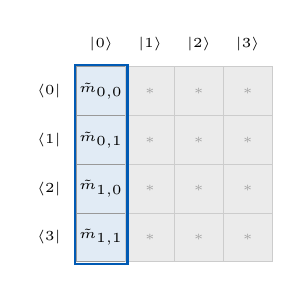
\begin{tikzpicture}[
      sig/.style={draw=black!40, fill=matrixfill,
                  minimum width=0.62cm, minimum height=0.62cm,
                  inner sep=0pt, font=\tiny, anchor=center},
      irr/.style={draw=black!20, fill=black!8,
                  minimum width=0.62cm, minimum height=0.62cm,
                  inner sep=0pt, font=\tiny, anchor=center,
                  text=black!35},
      klbl/.style={font=\tiny, text=black},
    ]
    \def\sz{0.62}
    %% draw 4x4 grid (schematic for PS=4, i.e. A is 2x2)
    \foreach \r in {0,...,3}{
      %% first column — signal (blue)
      \node[sig] (c\r-0) at (0, -\r*\sz) {};
      %% other columns — irrelevant (gray)
      \foreach \c in {1,...,3}{
        \node[irr] (c\r-\c) at (\c*\sz, -\r*\sz) {$\ast$};
      }
    }
    %% signal column entries
    \node[font=\tiny] at (c0-0) {$\tilde{m}_{0,0}$};
    \node[font=\tiny] at (c1-0) {$\tilde{m}_{0,1}$};
    \node[font=\tiny] at (c2-0) {$\tilde{m}_{1,0}$};
    \node[font=\tiny] at (c3-0) {$\tilde{m}_{1,1}$};
    %% column labels (top)
    \node[klbl, anchor=south] at ([yshift=2pt]c0-0.north) {$\ket{0}$};
    \node[klbl, anchor=south] at ([yshift=2pt]c0-1.north) {$\ket{1}$};
    \node[klbl, anchor=south] at ([yshift=2pt]c0-2.north) {$\ket{2}$};
    \node[klbl, anchor=south] at ([yshift=2pt]c0-3.north) {$\ket{3}$};
    %% row labels (left)
    \node[klbl, anchor=east] at ([xshift=-2pt]c0-0.west) {$\bra{0}$};
    \node[klbl, anchor=east] at ([xshift=-2pt]c1-0.west) {$\bra{1}$};
    \node[klbl, anchor=east] at ([xshift=-2pt]c2-0.west) {$\bra{2}$};
    \node[klbl, anchor=east] at ([xshift=-2pt]c3-0.west) {$\bra{3}$};
    %% blue highlight stripe
    \draw[matrixblue, thick]
      ([xshift=-0.5pt, yshift=0.5pt]c0-0.north west)
      rectangle
      ([xshift=0.5pt, yshift=-0.5pt]c3-0.south east);
    \end{tikzpicture}
    \subcaption{$\SP(M)$ for $M\in\mathbb{R}^{2\times 2}$ where $\tilde{m}_{i,j} = \frac{m_{i,j}}{\|M\|_F}$.}
    \label{fig:viz-sp}
  \end{minipage}
  \hfill
  %% ---- (b) SP(B)^dagger ----
  \begin{minipage}[t]{0.30\linewidth}
    \centering
    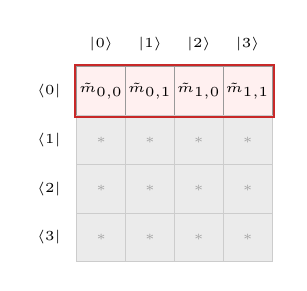
\begin{tikzpicture}[
      sig/.style={draw=black!40, fill=matrixfillred,
                  minimum width=0.62cm, minimum height=0.62cm,
                  inner sep=0pt, font=\tiny, anchor=center},
      irr/.style={draw=black!20, fill=black!8,
                  minimum width=0.62cm, minimum height=0.62cm,
                  inner sep=0pt, font=\tiny, anchor=center,
                  text=black!35},
      klbl/.style={font=\tiny, text=black},
    ]
    \def\sz{0.62}
    %% draw 4x4 grid
    \foreach \c in {0,...,3}{
      %% first row — signal (red)
      \node[sig] (d0-\c) at (\c*\sz, 0) {};
      %% other rows — irrelevant (gray)
      \foreach \r in {1,...,3}{
        \node[irr] (d\r-\c) at (\c*\sz, -\r*\sz) {$\ast$};
      }
    }
    %% signal row entries
    \node[font=\tiny] at (d0-0) {$\tilde{m}_{0,0}$};
    \node[font=\tiny] at (d0-1) {$\tilde{m}_{0,1}$};
    \node[font=\tiny] at (d0-2) {$\tilde{m}_{1,0}$};
    \node[font=\tiny] at (d0-3) {$\tilde{m}_{1,1}$};
    %% column labels (top)
    \node[klbl, anchor=south] at ([yshift=2pt]d0-0.north) {$\ket{0}$};
    \node[klbl, anchor=south] at ([yshift=2pt]d0-1.north) {$\ket{1}$};
    \node[klbl, anchor=south] at ([yshift=2pt]d0-2.north) {$\ket{2}$};
    \node[klbl, anchor=south] at ([yshift=2pt]d0-3.north) {$\ket{3}$};
    %% row labels (left)
    \node[klbl, anchor=east] at ([xshift=-2pt]d0-0.west) {$\bra{0}$};
    \node[klbl, anchor=east] at ([xshift=-2pt]d1-0.west) {$\bra{1}$};
    \node[klbl, anchor=east] at ([xshift=-2pt]d2-0.west) {$\bra{2}$};
    \node[klbl, anchor=east] at ([xshift=-2pt]d3-0.west) {$\bra{3}$};
    %% red highlight stripe
    \draw[matrixred, thick]
      ([xshift=-0.5pt, yshift=0.5pt]d0-0.north west)
      rectangle
      ([xshift=0.5pt, yshift=-0.5pt]d0-3.south east);
    \end{tikzpicture}
    \subcaption{$\SP(M)^\dagger$ for $M\in\mathbb{R}^{2\times 2}$ where $\tilde{m}_{i,j} = \frac{m_{i,j}}{\|M\|_F}$.}
  \end{minipage}
  \hfill
    %% ---- (b) MSP(B)^dagger ----
  \begin{minipage}[t]{0.30\linewidth}
    \centering
    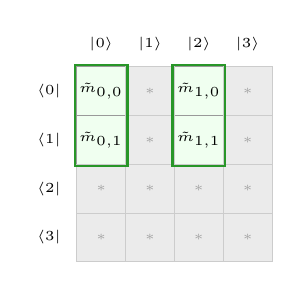
\begin{tikzpicture}[
      sig/.style={draw=black!40, fill=matrixfillgreen,
                  minimum width=0.62cm, minimum height=0.62cm,
                  inner sep=0pt, font=\tiny, anchor=center},
      irr/.style={draw=black!20, fill=black!8,
                  minimum width=0.62cm, minimum height=0.62cm,
                  inner sep=0pt, font=\tiny, anchor=center,
                  text=black!35},
      klbl/.style={font=\tiny, text=black},
    ]
    \def\sz{0.62}
    \node[sig] (d0-0) at (0, -0*\sz){};
    \node[sig] (d1-0) at (0, -1*\sz){};
    \node[sig] (d0-2) at (2*\sz, -0*\sz){};
    \node[sig] (d1-2) at (2*\sz, -1*\sz){};

    \foreach \c in {1,3}{
        \node[irr] (d0-\c) at (\c*\sz, -0*\sz) {$\ast$};
        \node[irr] (d1-\c) at (\c*\sz, -1*\sz) {$\ast$};
        \node[irr] (d2-\c) at (\c*\sz, -2*\sz) {$\ast$};
        \node[irr] (d3-\c) at (\c*\sz, -3*\sz) {$\ast$};
      }
    \node[irr] (d2-0) at (0*\sz, -2*\sz) {$\ast$};
     \node[irr] (d3-0) at (0*\sz, -3*\sz) {$\ast$};
     \node[irr] (d2-2) at (2*\sz, -2*\sz) {$\ast$};
      \node[irr] (d2-3) at (2*\sz, -3*\sz) {$\ast$};

    \node[font=\tiny] at (d0-0) {$\tilde{m}_{0,0}$};
    \node[font=\tiny] at (d1-0) {$\tilde{m}_{0,1}$};
    \node[font=\tiny] at (d0-2) {$\tilde{m}_{1,0}$};
    \node[font=\tiny] at (d1-2) {$\tilde{m}_{1,1}$};
    %% column labels (top)
    \node[klbl, anchor=south] at ([yshift=2pt]d0-0.north) {$\ket{0}$};
    \node[klbl, anchor=south] at ([yshift=2pt]d0-1.north) {$\ket{1}$};
    \node[klbl, anchor=south] at ([yshift=2pt]d0-2.north) {$\ket{2}$};
    \node[klbl, anchor=south] at ([yshift=2pt]d0-3.north) {$\ket{3}$};
    %% row labels (left)
    \node[klbl, anchor=east] at ([xshift=-2pt]d0-0.west) {$\bra{0}$};
    \node[klbl, anchor=east] at ([xshift=-2pt]d1-0.west) {$\bra{1}$};
    \node[klbl, anchor=east] at ([xshift=-2pt]d2-0.west) {$\bra{2}$};
    \node[klbl, anchor=east] at ([xshift=-2pt]d3-0.west) {$\bra{3}$};
    %% red highlight stripe
    \draw[matrixgreen, thick]
      ([xshift=-0.5pt, yshift=0.5pt]d0-0.north west)
      rectangle
      ([xshift=0.5pt, yshift=-0.5pt]d1-0.south east);
      \draw[matrixgreen, thick]
      ([xshift=-0.5pt, yshift=0.5pt]d0-2.north west)
      rectangle
      ([xshift=0.5pt, yshift=-0.5pt]d1-2.south east);
    \end{tikzpicture}
    \subcaption{$\MSP(M)$ for $M\in\mathbb{R}^{2\times 2}$ where $\tilde{m}_{i,j} = \frac{m_{i,j}}{\|M\|_F}$.}
  \end{minipage}
  \caption{Unitary matrices corresponding to
    \textbf{(a)}~$\SP(M)$,   \textbf{(b)}~$\SP(M)^\dagger$, and \textbf{(c)}~$\MSP(M)$
    shown schematically for $2\times 2$ matrix $M$.
    In $\SP(M)$, the first column (blue) contains the vectorised,
    Frobenius-normalised entries of $M$; the remaining columns (grey, marked $\ast$) are fixed by unitarity and play no role in the algorithm.
    In $\SP(M)^\dagger$, the first row (red) contains the normalised entries of $M$; the remaining rows are irrelevant. In $\MSP(M)$, the normalised entries (green) of $M$ retain the row structure of the original matrix.
    }
  \label{fig:viz}
\end{figure}

\Cref{fig:viz} illustrates the internal structure of the $\SP$, $\SP^\dagger$, and $\MSP$ unitaries for a concrete small matrix $M$. By \cref{def:sp}, the first column of $\SP(M)$ contains the vectorised, Frobenius-normalised entries of $M$; all remaining columns are fixed by unitarity but play no role in the algorithm. Dually, the first row of $\SP(M)^\dagger$ contains the normalised entries of $M$; all remaining rows are irrelevant. Finally, in $\MSP(M)$, the rows of the matrix $M$ are distributed among the columns with index a multiple of $R$. In particular, $\tilde m_{i,j}= \bra{0}^p\bra{j}^r\MSP(M)\ket{i}^p\ket{0}^r,$ with $i=0, \ldots, P-1$ and $j=0, \ldots, R-1.$ All remaining entries of $\MSP(M)$ are irrelevant. We observe that while the standard state-preparation operator $\SP(M)$ encodes the row-wise vectorization of the matrix $M$ into its first column, the modular state-preparation operator $\MSP(M)$ preserves the matrix's two-dimensional structure, encoding each row of $M$ in a separate column.

%% -----------------------------------------------------------------------
%% Section 3 — The Two-Tower Algorithm
%% -----------------------------------------------------------------------
\section{The Two-Tower Algorithm}
\label{sec:algorithm}
\begin{figure}[t]
  \centering
  \begin{quantikz}[wire types={b,b,b}, classical gap=0.07cm]
    \lstick{$\ket{0}^{n}$}
      & \qw
      & \swap{1}
      & \qw
      & \qw
      & \swap{1}
      & \qw
      & \qw \\
    \lstick{$\ket{0}^{m}$}
      & \gate[wires=2]{V(A)}
      & \targX{}
      & \gate[wires=2]{V(B^T)}
      & \gate[wires=2]{U(B^T)}
      & \targX{}
      & \gate[wires=2]{U(A)^\dagger}
      & \qw \\
    \lstick{$\ket{0}^{s}$}
      & \qw
      & \qw
      & \qw
      & \qw
      & \qw
      & \qw
      & \qw
  \end{quantikz}
  \caption{Original circuit for $C = AB$ from
    Bernasconi~et~al.~\cite{bernasconiMatMul}, with
    $A \in \mathbb{R}^{M \times N}$, $B \in \mathbb{R}^{N \times S}$,
    $m = \log M$, $n = \log N$, $s = \log S$.
    The circuit uses four state-preparation operators
    ($V(A)$, $U(A)^\dagger$, $V(B^T)$, $U(B^T)$)
    and %two swap gates.}
    performs two register swaps. }
  \label{fig:circuit-original}
\end{figure}
\begin{figure}[t]
  \centering
  \begin{quantikz}[wire types={b,b,b}, classical gap=0.07cm]
    \lstick{$\ket{0}^{s}$}
      & \qw\gategroup[3,steps=1,style={dotted, rounded corners, inner sep=1pt},label style={yshift=-3.8cm}]{$\OP(L)$}
      & \gate[wires=2]{\MSP(B)}\gategroup[3,steps=1,style={dotted, rounded corners, inner sep=1pt},label style={yshift=-3.8cm}]{$\OP(R)$}
      & \qw \\
    \lstick{$\ket{0}^{n}$}
      & \gate[wires=2]{\SP(A)}
      & \qw
      & \qw \\
    \lstick{$\ket{0}^{m}$}
      & \qw
      & \qw
      & \qw
  \end{quantikz}
  \caption{Circuit for computing $C = AB$, equivalent to
    \cref{fig:circuit-original} but reorganised into the Two-Tower
    two-layer structure $\OP(L)$ and $\OP(R)$.
    Layer~$\OP(L)$: $\SP(A) = U(A)  V(A)$ on registers
    $(n,m)$.
    Layer~$\OP(R)$: $\MSP(B)$ on registers $(s,n)$,
    a composite operator that applies the row-loading multiplexer
    $U(B)$ on $(s,n)$ followed by $V(B)^\dagger$ on $n$ to contract
    the shared index.
    This is the base case ($K=2$) of the Two-Tower construction.}
  \label{fig:circuit-2}
\end{figure}
This section presents the Two-Tower algorithm in two stages.
\Cref{sec:two_matrix} recalls the two-matrix subroutine
of~\cite{bernasconiMatMul}, which serves as the foundation. 
\Cref{sec:chain_mult} generalizes this construction to an arbitrary
chain of $K$ matrices. 


\subsection{Two-matrix multiplication}\label{sec:two_matrix}
In~\cite{bernasconiMatMul}, the authors introduce a quantum
subroutine for the product of two matrices
$A \in \mathbb{R}^{M \times N}$ and $B \in \mathbb{R}^{N \times S}$.
Their original circuit, shown in \cref{fig:circuit-original}, uses
operators $V(A)$, $U(A)^\dagger$, $V(B^T)$, $U(B^T)$ together with
two register swaps on quantum registers $\ket{0}^n$, $\ket{0}^m$, and $\ket{0}^s$.

We observe that this circuit can be rearranged
into the equivalent form shown in \cref{fig:circuit-2}, which serves
as the base case ($K = 2$) of the Two-Tower construction.
The key insight is that the composition
$U(A)^\dagger \, \,\mathrm{SWAP} \, U(B^T)  V(B^T) \, \, 
\mathrm{SWAP}\,  V(A)$ can be reorganised as the composition of 
$\MSP(B)$ and $\SP(A)$, eliminating the register swaps and
grouping the operators into two sequential layers acting on disjoint
register pairs. This reorganisation, while functionally identical for $K = 2$, reveals a two-layer structure --- denoted by $\OP(L)$ and $\OP(R)$ --- that generalises to arbitrary $K$. In particular, the rearranged circuit acts on $m + n + s$ qubits and produces:
\begin{equation*}
 (\mathbb{I}_M \otimes\MSP(B))\,(\SP(A)\otimes \mathbb{I}_S)\,\ket{0}^{m+n+s}
  = \frac{1}{\norm{A}_F\norm{B}_F}
    \sum_{i=0}^{M-1}\sum_{k=0}^{S-1}
    \underbrace{\sum_{j=0}^{N-1} a_{i,j}\,b_{j,k}}_{(AB)_{i,k}}
    \ket{i}^m\ket{0}^n\ket{k}^s + \ket{\bot},
\end{equation*}
encoding the product $AB$ in the outer registers with the internal
index contracted to $\ket{0}^n$ (see \cref{subsec:proof-even} for
a detailed derivation). 




\subsection{Chain multiplication for arbitrary \texorpdfstring{$K$}{K}}\label{sec:chain_mult}

The two-matrix construction of \cref{sec:two_matrix} generalises
naturally to an arbitrary chain of $K$ matrices
$\mathcal{W} = M^{(0)} M^{(1)} \cdots M^{(K-1)}$.
Before describing the full algorithm, we isolate the mechanism that
makes the construction work.

\subsubsection{The contraction mechanism}
Recall from \cref{def:sp} that $\SP(M)$ maps $\ket{0,0} \mapsto \frac{1}{\norm{M}_F}\sum_{i, j} m_{i, j}\ket{i, j}$. The adjoint $\SP(M)^\dagger$ reverses this map. Moreover, when $\SP(M)^\dagger$ acts on a basis state $\ket{i,j}$, it projects onto $\ket{0,0}$ with amplitude proportional to the corresponding matrix entry $m_{i,j}$. Formally,
\begin{equation}\label{eq:sp-collapse}
    \SP(M)^{\dagger}\,\ket{i,\,j}
    \;=\;
    \frac{m_{i,j}}{\norm{M}_F}\,\ket{0,0}
    \;+\; \ket{\bot}, \quad   0 \leq i < P, \text{ and } 0 \leq j < R,
\end{equation}
where $\ket{\bot}$ is orthogonal to $\ket{0,0}$. We observe that if two consecutive matrices $M^{(k)}$ and $M^{(k+1)}$ share a summation index encoded in the same quantum register, applying $\SP(M^{(k)})$ populates that register with amplitudes proportional to the entries of $M^{(k)}$, and $\SP(M^{(k+1)})^\dagger$ contracts it back to $\ket{0}$, multiplying each amplitude by the corresponding entry of $M^{(k+1)}$.
By linearity, all such combinations occur simultaneously, and the resulting amplitudes reproduce exactly the classical matrix product. The Two-Tower circuit arranges all matrices so that every shared index is contracted through this mechanism.

\subsubsection{Circuit structure}
The circuit consists of two parallel layers (see \cref{fig:circuit-K}):
$\OP(L)$ applies $\SP$ to every even-indexed matrix, and
$\OP(R)$ applies $\SP^\dagger$ to every odd-indexed matrix, with one exception: when $K$ is even, the last matrix $M^{(K-1)}$ has no paired right neighbour, and $\MSP(M^{(K-1)})$ is applied in place of $\SP(M^{(K-1)})^\dagger$ so that the output column register is preserved (see~\cref{def:MSP} and~\cref{fig:circuit-K-even}). Since the operators within each layer act on non-overlapping registers,
they execute in parallel, and the total circuit depth is independent
of $K$. Following the intuition from the matrix-product vectorization discussed in the introduction, these two layers realise the Kronecker products of the first and last matrices of each internal subchain; \cref{sec:algorithm:walkthrough} illustrates this in detail.

We observe that each matrix requires two registers to index rows and columns. However, registers are shared between adjacent matrices, so the overall circuit requires $K+1$  registers: two for the first matrix and one additional register for each remaining matrix.
Thus, the circuit grows in qubit count while its depth remains constant --- much like two towers rising floor by floor, which gives the algorithm its name. In~\cref{def:skyscraper-ops} we formalise the construction.

\begin{definition}[Two-Tower operators]\label{def:skyscraper-ops}
  Let $\mathcal{W} = M^{(0)}, \ldots, M^{(K-1)}$ be a matrix chain with $K \ge 2$.
   %, $K$ odd.
Partition the chain into:
  \begin{itemize}
    \item \emph{Left matrices} (even index):
          $M^{(2i)} \in \mathbb{R}^{L_i \times R_i}$, for
          $0 \leq i \leq \lfloor(K-1)/2\rfloor$;
    \item \emph{Right matrices} (odd index):
          $M^{(2j+1)} \in \mathbb{R}^{R_j \times L_{j+1}}$, for
          $0 \leq j \leq \lfloor(K/2 - 1)\rfloor$.
  \end{itemize}
  Let us define $l_i = \log L_i$ and $r_i = \log R_i$ for the qubit counts.
  For each left matrix allocate a register pair
  $\ket{0}^{l_i}\ket{0}^{r_i}$; the initial state is
  \begin{equation*}\label{eq:psi0}
    \ket{\psi_0}
    = \left\{\begin{array}{ll}
    \bigotimes_{i=0}^{(K-1)/2} \ket{0}^{l_i}\ket{0}^{r_i}, & \mbox{if $K$ is odd}\\
    \left(\bigotimes_{i=0}^{K/2-1} \ket{0}^{l_i}\ket{0}^{r_i}\right) \ket{0}^{l_{K/2}}, & \mbox{if $K$ is even.}
    \end{array}
    \right.
\end{equation*}
  The circuit uses $\sum_{i=0}^{(K-1)/2}(l_i + r_i)$ qubits if $K$ is odd and $\sum_{i=0}^{K/2-1}(l_i + r_i) + l_{K/2}$ if $K$ is even.
  Define:
  \begin{align}
    \OP(L) &= \left\{\begin{array}{ll}
    \bigotimes_{i=0}^{(K-1)/2} \SP\!\left(M^{(2i)}\right),& \mbox{if $K$ is odd}\\
    \bigotimes_{i=0}^{K/2-1} \SP\!\left(M^{(2i)}\right) \otimes \Id_{l_\frac{K}{2}}, & \mbox{if $K$ is even;}\\
    \end{array}
    \right.
    \label{eq:OPL}\\[4pt]
    \OP(R) &= \left\{\begin{array}{ll} \underbrace{\Id_{L_0}}_{\text{left boundary}}
              \otimes
              \underbrace{\bigotimes_{j=0}^{(K-3)/2} \SP\!\left(M^{(2j+1)}\right)^\dagger}_{\text{contracts shared indexes}}
              \otimes
              \underbrace{\Id_{R_{(K-1)/2}}}_{\text{right boundary}} & \mbox{if $K$ is odd}\\
              \underbrace{\Id_{L_0}}_{\text{left boundary}}
              \otimes
              \underbrace{\bigotimes_{j=0}^{K/2-2}\SP\!\left(M^{(2j+1)}\right)^\dagger}_{\text{contracts shared indexes}}
              \otimes \
              \underbrace{\MSP(M^{(K-1)})}_{\text{right boundary}} & \mbox{if $K$ is even}.
              \end{array}
    \right.
    \label{eq:OPR}
  \end{align}
  The \emph{Two-Tower unitary} is $U_\mathcal{W} = \OP(R)\OP(L)$.
\end{definition}

\begin{figure}[t]
  \centering

  %% ---- (a) K odd ----
  \begin{minipage}[b]{0.48\linewidth}
    \centering
    % 1) typeset the circuit into a box -- completely outside tikzpicture
    \newsavebox{\circOdd}%
    \sbox{\circOdd}{%
      \resizebox{\linewidth}{!}{%
        \begin{quantikz}[wire types={b,b,b,b,b,b,b,b}, classical gap=0.07cm]
                \lstick{$\ket{0}^{r_{\frac{K-1}{2}}}$} & \gate[wires=2]{\mathrm{SP}(M^{(K-1)})}\gategroup[8,steps=1,style={dotted,rounded corners,inner sep=1pt}, label style={yshift=-9.5cm}]{$\OP(L)$} & \gate[style={inner sep=2pt}]{\mathbb{I}_{R_{\frac{K-1}{2}}}}\gategroup[8,steps=1,style={dotted,rounded corners,inner sep=1pt}, label style={yshift=-9.5cm}]{$\OP(R)$} & \qw \\
                \lstick{$\ket{0}^{l_{\frac{K-1}{2}}}$} & \qw & \gate[wires=2]{\mathrm{SP}(M^{(K-2)})^{\dagger}} & \qw \\
                \lstick{$\ket{0}^{r_{\frac{K-1}{2}-1}}$} & \qw & \qw & \qw \\
                & \wave & \wave & \\
                \lstick{$\ket{0}^{r_1}$}
                & \gate[wires=2]{\mathrm{SP}(M^{(2)})} & \qw & \qw \\
                \lstick{$\ket{0}^{l_1}$} & \qw & \gate[wires=2]{\mathrm{SP}(M^{(1)})^{\dagger}} & \qw \\
                \lstick{$\ket{0}^{r_0}$} & \gate[wires=2]{\mathrm{SP}(M^{(0)})} & \qw & \qw \\
                \lstick{$\ket{0}^{l_0}$} & \qw & \gate[style={inner sep=2pt}]{\mathbb{I}_{L_0}} & \qw
        \end{quantikz}}%
    }%
    % 2) place the finished box inside tikzpicture -- no nesting, no extra groups
    \begin{tikzpicture}
      \node[inner sep=0pt, outer sep=0pt] (circ) {\usebox{\circOdd}};
      \begin{scope}[
          shift={(circ.south west)},
          x    ={($(circ.south east)-(circ.south west)$)},
          y    ={($(circ.north west)-(circ.south west)$)}]
        % [0,1]x[0,1] coordinate frame -- add annotations here

        \fill[white, opacity=1 ] (0.3, 0.75) rectangle (0.55, 0.65);
        \node at (0.425, 0.68){\scalebox{0.7}{$\mathrm{SP}(M^{(K-3)})$}};
        \draw[black, semithick] (0.3, 0.605) -- (0.3, 0.75) -- (0.55, 0.75) -- (0.55, 0.606);

        \fill[white, opacity=1] (0.65, 0.45) rectangle (0.9, 0.55);
        \node at (0.78, 0.52){\scalebox{0.9}{$\mathrm{SP}(M^{(3)})^{\dagger}$}};
        \draw[black, semithick] (0.65, 0.595) -- (0.65, 0.45) -- (0.9, 0.45) -- (0.9, 0.595);
                
      
      \end{scope}
    \end{tikzpicture}
    \subcaption{$K$ odd.}
    \label{fig:circuit-K-odd}
  \end{minipage}
  \hfill
  %% ---- (b) K even ----
  \begin{minipage}[b]{0.48\linewidth}
    \centering
    \newsavebox{\circEven}%
    \sbox{\circEven}{%
      \resizebox{\linewidth}{!}{%
        \begin{quantikz}[wire types={b,b,b,b,b,b,b,b}, classical gap=0.07cm]
                \lstick{$\ket{0}^{l_{\frac{K}{2}}}$} & \gate[style={inner sep=2pt}]{\mathbb{I}_{L_{\frac{K}{2}}}}\gategroup[8,steps=1,style={dotted,rounded corners,inner sep=1pt}, label style={yshift=-9.5cm}]{$\OP(L)$} & \gate[wires=2]{\MSP(M^{(K-1)})}\gategroup[8,steps=1,style={dotted,rounded corners,inner sep=1pt}, label style={yshift=-9.5cm}]{$\OP(R)$} & \qw \\
                \lstick{$\ket{0}^{r_{\frac{K}{2}-1}}$} & \gate[wires=2]{\mathrm{SP}(M^{(K-2)})} & \qw & \qw \\
                \lstick{$\ket{0}^{l_{\frac{K}{2}-1}}$} & \qw & \qw & \qw \\
                & \wave & \wave & \\
                \lstick{$\ket{0}^{r_1}$}
                & \gate[wires=2]{\mathrm{SP}(M^{(2)})} & \qw & \qw \\
                \lstick{$\ket{0}^{l_1}$} & \qw & \gate[wires=2]{\mathrm{SP}(M^{(1)})^{\dagger}} & \qw \\
                \lstick{$\ket{0}^{r_0}$} & \gate[wires=2]{\mathrm{SP}(M^{(0)})} & \qw & \qw \\
                \lstick{$\ket{0}^{l_0}$} & \qw & \gate[style={inner sep=2pt}]{\mathbb{I}_{L_0}} & \qw
        \end{quantikz}}%
    }%
    \begin{tikzpicture}
      \node[inner sep=0pt, outer sep=0pt] (circ) {\usebox{\circEven}};
      \begin{scope}[
          shift={(circ.south west)},
          x    ={($(circ.south east)-(circ.south west)$)},
          y    ={($(circ.north west)-(circ.south west)$)}]
        % [0,1]x[0,1] coordinate frame -- add annotations here
         
         \fill[white, opacity=1] (0.63, 0.75) rectangle (0.88, 0.63);
        \node at (0.755, 0.675){\scalebox{0.7}{$\mathrm{SP}(M^{(K-3)})^{\dagger}$}};
        \draw[black, semithick] (0.63, 0.62) -- (0.63, 0.75) -- (0.88, 0.75) -- (0.88, 0.62);

        \fill[white, opacity=1] (0.63, 0.45) rectangle (0.88, 0.55);
        \node at (0.76, 0.52){\scalebox{0.9}{$\mathrm{SP}(M^{(3)})^{\dagger}$}};
        \draw[black, semithick] (0.63, 0.595) -- (0.63, 0.45) -- (0.88, 0.45) -- (0.88, 0.595);
\draw[red, thick, dashed] 
    (0.2, 0.08) -- % Vertex 1 (Left-middle)
    (0.2, 0.875) -- % Vertex 2 (Top-left)
    (0.55, 0.875) -- % Vertex 3 (Top-right)
    (0.55, 0.765) -- % Vertex 4 (Right-middle)
    (0.96, 0.765) -- % Vertex 5 (Bottom-right)
    (0.96, 0.08) -- % Vertex 6 (Bottom-left)
    cycle;          % Closes the shape back to Vertex 1
      \end{scope}
    \end{tikzpicture}
    \subcaption{$K$ even.}
    \label{fig:circuit-K-even}
  \end{minipage}
  \caption{Two-Tower circuit for a chain of $K$ matrices.
    \textbf{(a)}~$K$ odd: registers are ordered top-to-bottom as
    $(r_{(K-1)/2},\, l_{(K-1)/2},\, \ldots,\, r_0,\, l_0)$.
    $\OP(L)$: all $\SP(M^{(2i)})$ act simultaneously on
    disjoint register pairs $(r_i, l_i)$.
    $\OP(R)$: all $\SP(M^{(2j+1)})^\dagger$ act simultaneously
    on the interleaved pairs $(l_{j+1}, r_j)$.
    \textbf{(b)}~$K$ even: an additional output register $l_{\frac{K}{2}}$
    appears at the top.
    The last matrix $M^{(K-1)}$ uses the $\MSP$ state preparation
    (denoted $\MSP(M^{(K-1)})$), which acts on
   $(l_{\frac{K}{2}},\, r_{K/2-1})$ within $\OP(R)$. This case can also be expressed as the product of two matrices: the result of applying the odd-case logic to the chain of the first $K-1$ matrices (dashed box in red), multiplied by the final matrix $M^{(K-1)}$ throught the $\MSP$ operator.}
  \label{fig:circuit-K}
\end{figure}

In $\OP(L)$, each $\SP(M^{(2i)})$ acts on the register pair $(\ket{0}^{l_i},\ket{0}^{r_i})$; all factors target disjoint registers and execute in parallel. In $\OP(R)$, each $\SP(M^{(2j+1)})^\dagger$ acts on the pair $(\ket{\,\cdot\,}^{r_j},\ket{\,\cdot\,}^{l_{j+1}})$ --- the boundary shared between adjacent even-matrix registers --- and, by \cref{eq:sp-collapse}, contracts it to $\ket{0}$, obtaining the corresponding entry of $M^{(2j+1)}$ as an amplitude up to a normalization factor. The identity operators $\Id_{L_0}$ and $\Id_{R_{(K-1)/2}}$ leave the outer indices $l_0$ and $r_{(K-1)/2}$ untouched; these encode the row and column indices of the product $\mathcal{W}$. The even-$K$ case (see \cref{fig:circuit-K-even}) requires $\MSP$ rather than $\SP^\dagger$ because $\SP^\dagger$ would contract both registers to $\ket{0}$, leaving no register to carry the output column index of $\mathcal{W}$; $\MSP$ contracts only the shared boundary register while keeping the output register free, yielding the same Frobenius-norm-scaled product.

\begin{algorithm}[t]
\caption{Two-Tower Matrix Multiplication}\label{alg:skyscraper}
\begin{algorithmic}[1]
  \Require Matrix chain $\mathcal{W} = (M^{(0)},\ldots,M^{(K-1)})$
           with $M^{(k)} \in \mathbb{R}^{P_k \times P_{k+1}}$, all dimensions powers of two.
  \Ensure Quantum state encoding $\mathcal{W} = M^{(0)}\cdots M^{(K-1)}$
          up to Frobenius-norm scaling.
  \State Allocate register $q_k$ of $\log P_k$ qubits for each
         $k = 0,\ldots,K-1$, and a final register $q_K$ of
         $\log P_K$ qubits; initialise all to $\ket{0}$.
    \State \textbf{Layer 1 (parallel).} For each even $k=2i,\;  0 \leq i \leq \lfloor(K-1)/2\rfloor$:
         apply $\SP(M^{(k)})$ on registers $(q_{k+1}, q_k)$.
    \State \textbf{Layer 2 (parallel).} For each odd $k=2j+1,\;  0 \leq j \leq\lceil K/2 -2\rceil$:
         apply $\SP(M^{(k)})^\dagger$ on registers $(q_{k+1}, q_k)$.
  \If{$K$ is even}
    \State Apply $\MSP(M^{(K-1)})$ on $(q_K, q_{K-1})$.
  \EndIf
  \State \Return The state $U_\mathcal{W}\ket{0} 
        $
        $q_0$ holds the row index of $\mathcal{W}$, $q_K$ holds the column index,
         and registers $q_1,\ldots,q_{K-1}$ are in state $\ket{0}$.
\end{algorithmic}
\end{algorithm}
\cref{alg:skyscraper} summarises the complete procedure; open-source Qiskit and QCLAB implementations are publicly available$^1$. 


\subsubsection{Two-Tower Algorithm Intuition}
\label{sec:algorithm:walkthrough}
The construction draws from a classical result in matrix theory. Lemma~4.3.1 of~\cite{horn2012matrix} expresses the product of three matrices via the Kronecker product and vectorization:
\begin{equation}\label{eq:horn}
AXB = C \quad\Longleftrightarrow\quad (B^T\otimes A)\,\text{vec}(X) = \text{vec}(C)
\end{equation}
In the quantum setting, preparing $A$ and $B$ on separate registers realises their Kronecker product naturally through the tensor-product structure of the Hilbert space. However, \cref{eq:horn} does not translate directly: $\SP(M)$ encodes any matrix in the statevector as a row-wise vectorization (\cref{eq:sp}), rather than as a matrix operator as~\cref{eq:horn} requires for $A$ and $B$. Consequently, whereas the classical formula $(B^T\otimes A)\,\text{vec}(X)$ yields exactly $\text{vec}(C)$, the Two-Tower circuit produces a higher-dimensional statevector containing $\text{vec}(C)$ alongside spurious contributions from index-mismatched combinations of entries of $A$, $X$, and $B$. A further difference is that the Two-Tower does not require any matrix transposition: each matrix is loaded directly through its own state-preparation operator, without reshaping $B$ into $B^T$. The contraction mechanism (\cref{eq:sp-collapse}) is what separates the two: $\SP(X)^\dagger$ projects the valid, index-matched contributions onto the $\ket{0}$ subspace of the shared registers, while all spurious terms fall into the orthogonal complement $\ket{\bot}$. To illustrate this filtering and observe how the correct sums accumulate, we trace the circuit of \cref{fig:circuit-3} for $D = ABC$ with $A \in \mathbb{R}^{M \times N}$, $B \in \mathbb{R}^{N \times S}$, $C \in \mathbb{R}^{S \times T}$. Let $m = \log M$, $n = \log N$, $s = \log S$, $t = \log T$, then we define the following quantum registers:
\begin{equation*}\label{eq:psi0-3}
  \ket{\psi_0} = \ket{0}^{m}\ket{0}^{n}\ket{0}^{s}\ket{0}^{t}.
\end{equation*}

\smallskip\noindent\textbf{Layer 1: apply $\OP(L) = \SP(A) \otimes \SP(C)$.}
Operator $\SP(A)$ acts on $(\ket{0}^{m}, \ket{0}^{n})$ while
$\SP(C)$ acts on $(\ket{0}^{s}, \ket{0}^{t})$ simultaneously:
\begin{equation*}\label{eq:psi1-3}
  \ket{\psi_1}= \OP(L)\ket{\psi_0}
  = \frac{1}{\norm{A}_F\norm{C}_F}
    \sum_{i=0}^{M-1}\sum_{j=0}^{N-1}\sum_{u=0}^{S-1}\sum_{v=0}^{T-1}
    a_{i,j}\, c_{u,v}\;\ket{i}^{m}\ket{j}^{n}\ket{u}^{s}\ket{v}^{t}.
\end{equation*}
\smallskip\noindent\textbf{Layer 2: apply $\OP(R) = \Id_M \otimes \SP(B)^\dagger \otimes \Id_T$.}
By \cref{eq:sp-collapse}, $\SP(B)^\dagger$ acts on registers $(n,s)$
picking up $\frac{b_{j, u}}{\norm{B}_F}$ for each basis state $\ket{j,u}$.
Applying to $\ket{\psi_1}$:
\begin{align*}
  \ket{\psi_2}=\OP(R)\ket{\psi_1}
  &= \frac{1}{\norm{A}_F\norm{B}_F\norm{C}_F}
     \sum_{i=0}^{M-1}\sum_{v=0}^{T-1}
     \Biggl(\sum_{j=0}^{N-1}\sum_{u=0}^{S-1}
       a_{i,j}\, b_{j,u}\, c_{u,v}
     \Biggr)\ket{i,0,0,v}
     + \ket{\bot}. \label{eq:OPR-psi1}
\end{align*}
The contraction of shared registers via \cref{eq:sp-collapse} is visible moving from
$\ket{\psi_1}$ to $\ket{\psi_2}$: $\SP(B)^\dagger$ projects each
basis state $\ket{j}^n\ket{u}^s$ onto $\ket{0}^n\ket{0}^s$ with
amplitude $\frac{b_{j,u}}{\norm{B}_F}$.
The indices $j$ and $u$ are summed over in the classical product
$(ABC)_{i, v} = \sum_{j,u} a_{i,j}\,b_{j,u}\,c_{u,v}$.
In the Two-Tower circuit, these sums arise from the superposition
over the shared registers $(n,s)$: the adjoint state preparation
$\SP(B)^\dagger$ converts each basis state $\ket{j,u}$ into the
corresponding matrix entry, and the superposition accumulates all
inner-product terms simultaneously.
As a result, the double sum over $(j,u)$ yields
$d_{i,v} = (ABC)_{i,v}$, confirming that $\ket{\psi_2}$ encodes $D$
in the outer registers $(m,t)$, with the shared registers $(n,s)$
contracted to $\ket{0,0}$.

\begin{figure}[t]
  \centering
  \begin{quantikz}[wire types={b,b,b,b}, classical gap=0.07cm]
    \lstick{$\ket{0}^{t}$} \slice{$\ket{\psi_0}$}
      & \gate[wires=2]{\SP(C)}\gategroup[4,steps=1,style={dotted, rounded corners, inner sep=1pt},label style={yshift=-5cm}]{$\OP(L)$} \slice{$\ket{\psi_1}$}
      & \gate[style={inner sep=2pt}]{\mathbb{I}_{T}}\gategroup[4,steps=1,style={dotted, rounded corners,inner sep=1pt},label style={yshift=-5cm}]{$\OP(R)$} \slice{$\ket{\psi_2}$}
      & \qw \\
    \lstick{$\ket{0}^{s}$}
      & \qw
      & \gate[wires=2]{\SP(B)^{\dagger}}
      & \qw \\
    \lstick{$\ket{0}^{n}$}
      & \gate[wires=2]{\SP(A)}
      & \qw
      & \qw \\
    \lstick{$\ket{0}^{m}$}
      & \qw
      & \gate[style={inner sep=2pt}]{\mathbb{I}_{M}}
      & \qw
  \end{quantikz}
  \caption{Two-Tower circuit for $D = ABC$ with
    $A \in \mathbb{R}^{M \times N}$, $B \in \mathbb{R}^{N \times S}$,
    $C \in \mathbb{R}^{S \times T}$,
    and $m = \log M$, $n = \log N$, $s = \log S$, $t = \log T$.
    \textbf{$\OP(L)$:} $\SP(C)$ on registers $(t,s)$ and $\SP(A)$
    on registers $(n,m)$ execute in \emph{parallel}.
    \textbf{$\OP(R)$:} $\SP(B)^\dagger$ on registers $(s,n)$ contracts the shared summation index.
    The output state $\ket{\psi_2}$ encodes $D$ in registers
    $(t,m)$ (outer boundaries) with the internal registers $(s,n)$ contracted to $\ket{0}$.}
  \label{fig:circuit-3}
\end{figure}
%% -----------------------------------------------------------------------
%% Section 4 — Analysis
%% -----------------------------------------------------------------------
\section{Analysis}
\label{sec:analysis}
We organize this section as follows: 
\Cref{subsec:correctness} proves that the Two-Tower circuit correctly
encodes the chain product for any $K$.
\Cref{subsec:complexity-analysis} derives the depth and qubit bounds.
\Cref{subsec:normalisation-signal} discusses the normalisation factor and 
the signal weight.

%%-----------------------------------------------------------------------
\subsection{Correctness}\label{subsec:correctness}
The correctness proof relies on the contraction mechanism of
\cref{eq:sp-collapse}, established in \cref{sec:chain_mult}.
The main result follows.

\begin{theorem}[Two-Tower Matrix Multiplication]\label{thm:main}
  Let $\mathcal{W} = M^{(0)}, \ldots, M^{(K-1)}$ be a matrix chain with $M^{(k)}\in \mathbb{R}^{P_k \times P_{k+1}}$ for $k = 0, \ldots, K-1$,
  and with all $p_k=\log_2P_k$.
  There exists a unitary $U_\mathcal{W} = \OP(R)\,\OP(L)$ such that
  \begin{equation}\label{eq:main-mapping}
  \begin{aligned}
    &U_\mathcal{W} \;\colon\;
    \ket{0}^{p_0}\ket{0}^{p_1+\cdots+p_{K-1}}\ket{0}^{p_K}
    \\
    &\;\longmapsto\;
    \frac{1}{\prod_{k=0}^{K-1}\norm{M^{(k)}}_F}
    \sum_{p=0}^{P_0-1}\sum_{q=0}^{P_K-1}
      w_{p,q}\,
      \ket{p}^{p_0}\ket{0}^{p_1+\cdots+p_{K-1}}\ket{q}^{p_{K}}
    + \ket{\bot},
  \end{aligned}
  \end{equation}
  where $\mathcal{W} = M^{(0)} \cdots M^{(K-1)}$ and $w_{p,q} = (\mathcal{W})_{p,q}$.
  The term $\ket{\bot}$ is a superposition
  of basis states in which at least one intermediate (shared) register
  is not $\ket{0}$; it is orthogonal to the subspace
  $\mathcal{H}_{\mathcal{W}} = \mathrm{span}\{\lvert p,0,\ldots,0,q \rangle \}$ for $0\le p < P_0,\; 0\le q < P_K$
  The circuit $U_\mathcal{W}$ has:
  \begin{itemize}
    \item \textbf{Depth}
          $\mathcal{O}\!\bigl(\max_{k=0}^{K-1} {\,\mathrm{polylog}}(P_k P_{k+1})\bigr)$, independent of $K$;
    \item \textbf{Qubits}
          $O\!\bigl(\sum_{k=0}^{K} \log P_k\bigr)$.
  \end{itemize}
\end{theorem}

\begin{proof}[Proof of \cref{thm:main} for odd $K$]\label{subsec:proof-odd}
Using the notation of \cref{sec:chain_mult}: left matrices
$M^{(2i)} \in \mathbb{R}^{P_k \times P_{k+1}}$ (where $k = 2i$) and right matrices
$M^{(2j+1)} \in \mathbb{R}^{ P_{k+1} \times  P_{k+2}}$  (where $k = 2j$), with shared registers shared between adjacent pairs. 

\smallskip\noindent\textbf{Step~1.}
Since all factors of $\OP(L) = \bigotimes_i \SP(M^{(2i)})$ act on
disjoint registers:
\begin{equation*}\label{eq:psi1-gen}
  \ket{\psi_1} = \frac{1}{\prod_i \norm{M^{(2i)}}_F}
    \!\!\sum_{\vec{l},\vec{r}}
    \!\!\left(\prod_i m^{(2i)}_{l_i,r_i}\right)
    \ket{l_0}\ket{r_0,\,l_1,\, r_1,\ldots,r_{(K-1)/2-1}\,l_{(K-1)/2}}\ket{r_{(K-1)/2}}.
\end{equation*}

\smallskip\noindent\textbf{Step~2.}
By \cref{eq:sp-collapse}, each $\SP(M^{(2j+1)})^\dagger$ on shared pair
$\ket{r_j, l_{j+1}}$ contributes amplitude
$\frac{m^{(2j+1)}_{r_j,l_{j+1}}}{\norm{M^{(2j+1)}}_F}$ on $\ket{0,0}$.
Applying all $(K-1)/2$ such operators in parallel and collecting:
\begin{equation*}\label{eq:OPR-psi1-gen}
  \OP(R)\ket{\psi_1}
  = \frac{1}{\prod_{k} \norm{M^{(k)}}_F}
    \sum_{\vec{l},\vec{r}}
    \!\!\left(\prod_i m^{(2i)}_{l_i,r_i}\right)
    \!\!\left(\prod_j m^{(2j+1)}_{r_j,l_{j+1}}\right)
    \ket{l_0,\underbrace{0,\ldots,0}_{\text{shared}},r_{(K-1)/2}}
    + \ket{\bot}.
\end{equation*}
\noindent Observing that 
$$
   \sum_{\vec{l},\vec{r}}
    \!\!\left(\prod_{i} m^{(2i)}_{l_i,r_i}\right)
    \!\!\left(\prod_j m^{(2j+1)}_{r_j,l_{j+1}}\right)=  \!\!\sum_{r_0,l_1,\ldots,l_{(K-1)/2}}
  \!\!m^{(0)}_{l_0,r_0}\cdots m^{(K-1)}_{l_{(K-1)/2},r_{(K-1)/2}}
  = w_{l_0,\,r_{(K-1)/2}}\;,
$$
and setting
$p \leftarrow l_0$, $q \leftarrow r_{(K-1)/2}$
yields~\cref{eq:main-mapping}.
\end{proof}

%%-----------------------------------------------------------------------

When $K$ is even, the chain contains $K/2$ even-indexed matrices ${M^{(0)}, M^{(2)}, \ldots, M^{(K-2)}}$ and $K/2$ odd-indexed matrices ${M^{(1)}, M^{(3)}, \ldots, M^{(K-1)}}$. The last odd-indexed matrix $M^{(K-1)}$ has no paired right neighbour, so a plain $\SP(M^{(K-1)})^{\dagger}$ would contract both registers to $\ket{0}$, leaving no register to carry the output column index. Instead, we encode $M^{(K-1)}$ via the modular state-preparation operator $\MSP(M^{(K-1)})$.

\begin{proof}[Proof of \cref{thm:main} for even $K$]\label{subsec:proof-even}
Apply the odd-$K$ argument of \cref{subsec:proof-odd} to the first $K-1$
matrices (an odd-length chain).
Then, we append a fresh ancilla register of $p_K=\log_2 P_K$ qubits for the
final column index.
The intermediate state after processing the first $K-1$ matrices of the chain $Z= M^{(0)}\cdots M^{(K-2)}$ is:
\begin{equation*}\label{eq:psi-half}
  \ket{\psi_{1}}
  = \frac{1}{\prod_{k=0}^{K-2}\norm{M^{(k)}}_F}
    \sum_{l_0=0}^{P_0-1}\sum_{d=0}^{P_{K-1}-1}
    z_{l_0,d}\,
\ket{l_0,\underbrace{0,\ldots,0}_{\text{shared}},d,\underbrace{0}_{\text{ancilla}}}
    \;+\; \ket{\bot},
\end{equation*}
where $z_{l_0,d} = (M^{(0)}\cdots M^{(K-2)})_{l_0,d}$ and the ancilla register remains in state $\ket{0}$. Projecting $\ket{\psi_{1}}$ onto the outer registers $(p_0, p_{K-1})$ yields exactly $\SP(Z)$. We then complete the chain product by applying the modular state-preparation operator $\MSP(M^{(K-1)})$ as in the two-matrix circuit of \cref{sec:two_matrix}, since $\mathcal{W} = Z M^{(K-1)}$.
\end{proof}

%%-----------------------------------------------------------------------

\subsection{Complexity}\label{subsec:complexity-analysis}
The depth and qubit bounds stated in \cref{thm:main} derive from the structure of the two-layer circuit and the state-preparation cost. In particular:

\begin{itemize}
  \item \textbf{Depth.} Each $\SP(M^{(k)})$ and $\SP(M^{(k)})^\dagger$ has depth $\mathcal{O}({\mathrm {polylog}}(P_kP_{k+1}))$. Since all even-indexed $\SP$ operators execute in parallel on the first layer, and all odd-indexed $\SP^\dagger$ operators execute in parallel on the second layer, the total depth is $\mathcal{O}(\max_{k} {\mathrm {polylog}}(P_k P_{k+1}))$, independent of $K$.
  \item \textbf{Qubits.} The circuit allocates one register of $p_k=\log_2 P_k$ qubits for each matrix $M^{(k)}$, $k=0,\ldots,K-1$, and a final register  $p_K=\log_2 P_K$ qubits for the output column index. Adjacent matrices share a shared register already counted in the allocation for $M^{(k+1)}$, and no additional ancillae are required. The total is $\sum_{k=0}^{K} \log_2 P_k = \Theta\!\bigl(\sum_{k=0}^{K} \log_2 P_k \bigr)$.   
\end{itemize}


%%-----------------------------------------------------------------------
\subsection{Normalisation and signal weight}\label{subsec:normalisation-signal}
The amplitudes in~\cref{eq:main-mapping} carry the \emph{normalisation factor} $\mathcal{N} = \frac{1}{\prod_{k=0}^{K-1} \norm{M^{(k)}}_F}$, which we compute classically before running the circuit. The residual term $\ket{\bot}$ lies in the orthogonal complement of $\mathcal{H}_{\mathcal{W}} = \mathrm{span}\{ \lvert p,0,\ldots,0,q \rangle \}$ for $0 \leq p < P_0$ and $0 \leq q < P_K$ and has squared norm $1 - \norm{\mathcal{W}}_F^2 \mathcal{N}^2$; this term does not indicate a failure of the subroutine but is the component of the unitary evolution that falls outside the subspace encoding the product. We therefore define the \emph{signal weight} as the total squared amplitude carried by the basis states in $\mathcal{H}_{\mathcal{W}}$ --- those whose amplitudes, up to the normalisation factor $\mathcal{N}$, are exactly the entries of the chain product:
$$
\Omega_{\mathcal{W}}
= \frac{\norm{\mathcal{W}}_F^2}{\prod_{k=0}^{K-1} \norm{M^{(k)}}_F^2}.
$$
In a standalone algorithm, $\Omega_{\mathcal{W}}$ would correspond to the success probability of post-selecting on $\mathcal{H}_\mathcal{W}$. However, the Two-Tower --- much like the QFT --- is designed as a subroutine with a downstream algorithm applied before any measurement; we therefore use the term \emph{signal weight} to emphasise that $\Omega_{\mathcal{W}}$ is a parameter inherited by the subsequent computation, not a measurement outcome of the circuit itself. 


For example a  special case where $\Omega_{\mathcal{W}}$ is absorbed analytically is the estimation  of $\|\mathcal{W}\|_F$: since $\Omega_{\mathcal{W}} = \|\mathcal{W}\|_F^2 / \prod_k \|M^{(k)}\|_F^2
$ and the denominator is classically known, Amplitude Estimation %of the post-selection probability 
directly yields $\|\mathcal{W}\|_F$ without any penalty from the signal weight. 
%Other cases of absortion are for example the computation of ${\rm trace}(\mathcal{W})$ or the computation  of normalized inner products.

By sub-multiplicativity of the Frobenius norm
($\norm{AB}_F \leq \norm{A}_F \norm{B}_F$),
$\Omega_{\mathcal{W}} \leq 1$, with $\Omega_{\mathcal{W}} = 1$ if and only
if $\|\mathcal{W}\|_F= \prod_{k=0}^{K-1} \|M^{(k)}\|_F$, and this happens in special cases. For example, consider $K$ copies of a normal $N \times N$ matrix $A$, i.e., a matrix such that  $A^\dagger A=AA^\dagger$ and denote its singular values by
$\sigma_1 \geq \cdots \geq \sigma_N \ge 0$.
Since $\norm{A}_F^2 = \sum_i \sigma_i^2$ and singular values of $\mathcal{W} = A^K$ when $A$ is normal are $\sigma_i^K$,  we get  
$\norm{A^K}_F^2 = \sum_i \sigma_i^{2K}$.  The signal weight becomes
$$
  \Omega_{\mathcal{W}}
  = \frac{\norm{A^K}_F^2}{\norm{A}_F^{2K}}
  = \frac{\sum_i \sigma_i^{2K}}{(\sum_i \sigma_i^2)^K},
$$
which for large $K$ is dominated by the largest singular value:
$\Omega_{\mathcal{W}} \approx (\sigma_1^2 / \norm{A}_F^2)^{K-1}$.
In general, $\Omega_{\mathcal{W}}$ can decrease with $K$; the rate of decay depends on the spectral structure of the matrices.
Two edge cases are instructive.
\begin{itemize}
  \item \emph{Well-conditioned matrices}
    ($\sigma_1/\sigma_N \approx 1$): all singular values are
    approximately equal to the same  $\sigma$, so
    $\|A^K\|_F^2 / \norm{A}_F^2 \approx N\,\sigma^{2K} / (N\sigma^2)^K
    $, giving $\Omega_{\mathcal{W}} \approx N^{-(K-1)}$. The signal weight decays exponentially with $K$: the information spreads across many directions and repeated multiplication reduces the overall signal strength. Note that the unitary case ($\sigma = 1$) belongs to this category, since $\Omega_{\mathcal{W}} = N/N^K = 1/N^{K-1}$.
  \item \emph{Near-rank-one matrices}
    ($\sigma_2 \approx 0$): a single singular value dominates the Frobenius norm, so $\Omega_{\mathcal{W}} \approx \frac{\sigma_1^{2K}}{\norm{A}_F^{2K}} \approx 1$. The matrix acts essentially as a scalar along one direction, and repeated multiplications do not weaken the signal.
\end{itemize}
The signal weight is therefore data-dependent: matrices with flat spectra cause rapid decay, whereas matrices with peaked spectra maintain $\Omega_{\mathcal{W}}$ close to unity. This phenomenon is counterintuitive: in most numerical settings, well-conditioned matrices are the favorable case, but here a flat spectrum spreads the signal uniformly across all singular directions, diluting it exponentially with $K$. Nevertheless, we observe that Amplitude Amplification~\cite{brassard2002quantum} can boost $\Omega_{\mathcal{W}}$ to any desired constant, at the cost of $\mathcal{O}(1/\sqrt{\Omega_{\mathcal{W}}})$ calls to the Two-Tower circuit and its inverse, introducing a dependence on $K$. 
%For $N \times N$ matrices, each call has depth $\mathcal{O}(\max_k \mathrm{polylog}(N))$, so the total depth after amplification becomes
%$$
%\mathcal{O}\left(
%\frac{\prod_k \norm{M^{(k)}}_F}{\norm{\mathcal{W}}_F}
%\,\mathrm{polylog}(N)
%\right).
%$$
%The amplification factor $\prod_k \norm{M^{(k)}}_F / \norm{\mathcal{W}}_F = 1/\sqrt{\Omega_{\mathcal{W}}}$ can grow with $K$, as the spectral discussion above shows. %The circuit depth of \cref{thm:main} is therefore $K$-independent, but the amplified depth may not be. In the worst case (well-conditioned matrices), Amplitude Amplification reintroduces a $K$-dependent cost, and any comparison with $O(K\,\mathrm{polylog}(N))$ block-encoding approaches~\cite{chakraborty_et_al:LIPIcs.ICALP.2019.33} must account for this tradeoff. 


%% -----------------------------------------------------------------------
%% Section 5 — Matrix-Chain-Vector Multiplication
%% -----------------------------------------------------------------------
\section{Matrix-Chain-Vector Multiplication}
\label{sec:vector}
An important special case of \cref{thm:main} arises when the last matrix in the chain is a column vector. This case finds direct application in iterative solvers, the power method, and Krylov subspace methods~\cite{GolubVanLoan1996}, all of which require repeated matrix-vector products. The following corollary formalises this specialisation.

\begin{corollary}[Matrix-chain-vector multiplication]\label{cor:vector-case}
  Setting $P_K = 1$ in \cref{thm:main} identifies $M^{(K-1)}$ with
  a column vector $v \in \mathbb{R}^{P_{K-1}}$.
  The right-boundary register vanishes ($\log 1 = 0$ qubits), and
  the Two-Tower encodes the product
  $w = M^{(0)}\cdots M^{(K-2)}\,v \in \mathbb{R}^{P_0}$
  as the amplitudes of the $\log P_0$-qubit output register, in
  depth $\mathcal{O}(\max_k {\mathrm {polylog}}(P_k P_{k+1}))$ using
  $\Theta\!\bigl(\sum_{k=0}^{K-1} \log P_k \bigr)$
  qubits.
\end{corollary}
\begin{proof}
  Immediate from \cref{thm:main} with $P_K = 1$: the
  $\log_2 P_K= 0$ qubits vanish from both the register allocation
  and the output state, and all remaining bounds carry over unchanged.
\end{proof}

\begin{figure}[t]    
  \centering
  \begin{quantikz}[wire types={b,b,b,b}, classical gap=0.07cm]
    \lstick{$\ket{0}^{t}$}
      & \gate[wires=2]{\SP(C)}\gategroup[4,steps=1,style={dotted, rounded corners, inner sep=1pt},label style={yshift=-5cm}]{$\OP(L)$}
      & \gate[style={inner sep=2pt}]{\SP(v)^{\dagger}}\gategroup[4,steps=1,style={dotted, rounded corners, inner sep=1pt},label style={yshift=-5cm}]{$\OP(R)$}
      & \qw \\
    \lstick{$\ket{0}^{s}$}
      & \qw
      & \gate[wires=2]{\SP(B)^{\dagger}}
      & \qw \\
    \lstick{$\ket{0}^{n}$}
      & \gate[wires=2]{\SP(A)}
      & \qw
      & \qw \\
    \lstick{$\ket{0}^{m}$}
      & \qw
      & \gate[style={inner sep=2pt}]{\mathbb{I}_{M}}
      & \qw
  \end{quantikz}    
  \caption{Chain-vector circuit for $w = ABCv$ with
    $A \in \mathbb{R}^{M \times N}$, $B \in \mathbb{R}^{N \times S}$,
    $C \in \mathbb{R}^{S \times T}$, $v \in \mathbb{R}^{T \times 1}$.
    Since $P_K= 1$, the output register vanishes and the
    $\MSP$ decomposition of the last factor reduces to
    $\SP(v)^\dagger$ on the $t$-qubit boundary register alone.
    The product $w = ABCv \in \mathbb{R}^{M}$ is encoded
    in the $m$-qubit register, with all shared registers $(t,s,n)$
    contracted to $\ket{0}$.}
    \label{fig:circuit-vector}
\end{figure}

We validate this specialisation at machine precision using open-source Qiskit and QCLAB implementations$^1$, confirming that the circuit correctly produces the chain-vector product for all tested instances. \Cref{fig:circuit-vector} illustrates the case $K=4$ with $w = ABCv$: the column-index register is no longer needed and $\MSP(v)$ reduces to $\SP(v)^\dagger$ on the boundary register alone, so the product vector is encoded entirely in the bottom register.



%% -----------------------------------------------------------------------
%% Section 6 — Conclusions and Future Work
%% -----------------------------------------------------------------------
\section{Conclusions and Future Work}
\label{sec:conclusions}
We presented the Two-Tower Matrix Multiplication, a quantum subroutine that encodes $\mathcal{W} = M^{(0)}\cdots M^{(K-1)}$, $M^{(k)}\in \mathbb{R}^{P_k\times P_{k+1}}$, using $\Theta\bigl(\sum_{k=0}^{K} \log P_k \bigr)$ qubits and circuit depth $\mathcal{O}(\max_k \mathrm{polylog}(P_k P_{k+1}))$, independent of $K$. The construction generalises the two-matrix operators of~\cite{bernasconiMatMul} to arbitrary chain length by interleaving $\SP$ and $\SP^\dagger$ gates on disjoint registers; the $\SP^\dagger$ contraction drives all shared registers to $\ket{0}$, producing the chain product as amplitudes.
Compared with classical algorithms, the Two-Tower trades sequential $\mathcal{O}(K \cdot N^\omega)$ depth --- or $\mathcal{O}(\log K \cdot \log N)$ with unbounded parallelism --- for $\mathcal{O}(\mathrm{polylog}(N))$ quantum depth. The advantage materialises when the downstream computation requires only aggregate quantities of $\mathcal{W}$ extractable via Amplitude Estimation. Representative instances include: norm, trace, and variance estimation via Amplitude Estimation~\cite{antonioli2025outlier,bernasconi2024quantum,cade2017quantum,poggiali2023quantum};
graph-matrix powers $A^K$ for spectral analysis, walk counting, and
mixing estimation~\cite{nghiem2023quantum,janzing610235bqp};
linear systems with chain-structured operators via
HHL~\cite{harrow2009quantum} or Neumann-series
LCU~\cite{chakraborty_et_al:LIPIcs.ICALP.2019.33};
and kernel evaluation in quantum machine
learning~\cite{biamonte2017quantum,kerenidis_et_al:LIPIcs.ITCS.2017.49}.
The chain-vector specialisation opens connections to iterative
numerical methods --- including the power method ($A^t v$), Krylov
subspace construction ($\{v, Av, \ldots, A^{t-1}v\}$), iterative
refinement via Neumann series, and polynomial matrix evaluation
$p(A)v$ --- where the Two-Tower provides a depth-efficient
building block for each matrix-vector product in the iteration.

Several directions for future work emerge from the present
construction.

\begin{itemize}
\item \emph{Trading depth for width.}
As shown in \cref{subsec:normalisation-signal}, the signal weight $\Omega_{\mathcal{W}}$ can decrease with the chain length $K$. A natural mitigation is a \emph{hybrid strategy} that alternates between the Two-Tower and block-encoding: the Two-Tower computes partial chain products in constant depth at the cost of growing qubit count and decaying signal weight, while block-encoding stages absorb the intermediate results and continue the multiplication in depth rather than width. This approach trades qubit overhead for circuit depth within the same computation, but it requires an efficient conversion between statevector encoding and block encoding --- an open problem that we leave for future investigation.

\item \emph{Complex matrices.}
The current construction assumes real entries. Extending to complex-valued matrices requires loading the entry-wise conjugate $\overline{M^{(k)}}$ in place of $M^{(k)}$ within $\OP(R)$, so that the contraction mechanism produces the correct Hermitian inner products; the rest of the circuit remains unchanged. A formal proof and numerical validation are left for future work.

\item \emph{Unitary chain encoding.}
An interesting generalisation replaces the matrices $M^{(0)}, M^{(1)},\ldots,$ $ M^{(K-1)}$ with arbitrary unitary operators $U_0, \ldots, U_{K-1}$, encoding their product as a quantum state. Each $U_k$ would enter the circuit through a state-preparation oracle that places the vectorized unitary in its first column. If the contraction mechanism extends to this setting, the Two-Tower could compute transition amplitudes $\bra{\phi} U_0 \cdots U_{K-1} \ket{v}$ at depth independent of $K$, with direct applications in quantum simulation and process tomography. We leave the formal analysis of this direction for future work.
\end{itemize}

%% -----------------------------------------------------------------------
%% Bibliography
%% -----------------------------------------------------------------------
\bibliography{main}



\end{document}

%% -----------------------------------------------------------------------
%% Appendix — Detailed Proofs
%% -----------------------------------------------------------------------

\begin{comment}

\appendix

\section{Detailed Proof for Three Matrices}
\label{app:proof-three}

We give a fully explicit computation for the case $K=3$,
$D = ABC$ with $A \in \mathbb{R}^{M \times N}$,
$B \in \mathbb{R}^{N \times S}$, $C \in \mathbb{R}^{S \times T}$,
using registers $m = \log M$, $n = \log N$, $s = \log S$,
$t = \log T$ and circuit as in \cref{fig:circuit-3}.

\begin{proof}[Proof for three matrices $D = ABC$]
Define the initial state:
\begin{align*}
    \ket{\psi_0} = \ket{0}^{m}\ket{0}^{n}\ket{0}^{s}\ket{0}^{t}.
\end{align*}
Apply $\SP(A)$ to $\ket{0}^{m}\ket{0}^{n}$ and $\SP(C)$ to
$\ket{0}^{s}\ket{0}^{t}$ simultaneously:
\begin{align*}
    \ket{\psi_1}
    &= \frac{1}{\| A \|_F}\sum_{i=0}^{M-1}\sum_{j=0}^{N-1}
       a_{i,j}\ket{i}^{m}\ket{j}^{n}
       \otimes
       \frac{1}{\| C \|_F}\sum_{u=0}^{S-1}\sum_{v=0}^{T-1}
       c_{u,v}\ket{u}^{s}\ket{v}^{t}\\
    &= \frac{1}{\| A \|_F\| C \|_F}
       \sum_{i,j,u,v}
       a_{i,j} \cdot c_{u,v}\,\ket{i,j,u,v}.
\end{align*}

Next, write $\SP(B)^{\dagger}$ explicitly using
\cref{eq:sp-collapse}:
\begin{align*}
\SP(B)^{\dagger}
= \frac{1}{\| B\|_F}
    \sum_{w=0}^{N-1}\sum_{z=0}^{S-1}
    b_{w,z}\,\ket{0,0}\bra{w,z}
    \;+\; \ket{\bot}\bra{\bot},
\end{align*}
where $\ket{\bot}\bra{\bot}$ collects all terms mapping onto states
orthogonal to $\ket{0,0}$.
The full second-layer operator is:
\begin{align*}
    \OP(R)
    &= \Id_M \otimes \SP(B)^{\dagger} \otimes \Id_T \\
    &= \sum_{f=0}^{M-1} \ket{f}\bra{f}
       \otimes \SP(B)^{\dagger}
       \otimes \sum_{g=0}^{T-1} \ket{g}\bra{g}.
\end{align*}
Using the tensor product rule
$(\ket{a}\bra{b}) \otimes (\ket{c}\bra{d}) = \ket{a,c}\bra{b,d}$,
we expand:
\begin{align*}
   \OP(R)
   = \frac{1}{\| B\|_F}
     \sum_{f,w,z,g}
     b_{w,z}\,\ket{f,0,0,g}\bra{f,w,z,g}
     \;+\; \ket{\bot}\bra{\bot}.
\end{align*}

Now apply $\OP(R)$ to $\ket{\psi_1}$.
The \replaced[id=GA]{contract}{collapse} mechanism (\cref{eq:sp-collapse}) enforces
$\braket{f,w,z,g}{i,j,u,v}
= \delta_{fi}\,\delta_{wj}\,\delta_{zu}\,\delta_{gv}$,
selecting matching indices and yielding:
\begin{align*}
    \OP(R)\ket{\psi_1}
    = \frac{1}{\| A \|_F\| B\|_F\| C \|_F}
      \sum_{f=0}^{M-1}\sum_{g=0}^{T-1}
      \Biggl(
        \sum_{w=0}^{N-1}\sum_{z=0}^{S-1}
        a_{f,w} \cdot b_{w,z} \cdot c_{z,g}
      \Biggr)
      \ket{f,0,0,g}
      + \ket{\bot}.
\end{align*}
Recognising $d_{f,g}
= \sum_{w}\sum_{z} a_{f,w}\, b_{w,z}\, c_{z,g}
= (ABC)_{f,g}$, we conclude:
\begin{align*}
    \ket{\psi_2}
    = \frac{1}{\| A \|_F\| B\|_F\| C \|_F}
      \sum_{f=0}^{M-1}\sum_{g=0}^{T-1}
      d_{f,g}\,\ket{f, 0, 0, g}
      + \ket{\bot},
\end{align*}
confirming that the circuit of \cref{fig:circuit-3}
encodes $D = ABC$ in the outer registers $(m, t)$
with the shared registers $(n, s)$ \replaced[id=GA]{contracted}{collapsed} to $\ket{0,0}$.
\end{proof}


\section{Detailed Proof for a Chain of \texorpdfstring{$K$}{K} Matrices (Odd \texorpdfstring{$K$}{K})}
\label{app:proof-K}

We extend the computation to a chain of $K$ matrices
$\mathcal{W} = M^{(0)} M^{(1)} \cdots M^{(K-1)}$ with $K$ odd,
using the notation of \cref{sec:chain_mult}:
left matrices
$L = \{M^{(2i)} \in \mathbb{R}^{L_i \times R_i}\}_{i=0}^{(K-1)/2}$
with entries $m^{(2i)}_{l_i, r_i}$,
and right matrices
$R = \{M^{(2j+1)} \in \mathbb{R}^{R_j \times L_{j+1}}\}_{j=0}^{\lfloor(K-2)/2\rfloor}$
with entries $m^{(2j+1)}_{r_j, l_{j+1}}$.

\begin{proof}[Proof of \cref{thm:main} for odd $K$ --- detailed version]
The initial state is:
\begin{align*}
    \ket{\psi_0}
    = \bigotimes_{i=0}^{(K-1)/2}
      \ket{0}^{\log L_i}\ket{0}^{\log R_i}.
\end{align*}

\smallskip\noindent\textbf{Step 1: Apply $\OP(L)$.}
Since $\OP(L) = \bigotimes_{i=0}^{(K-1)/2} \SP(M^{(2i)})$
and all factors act on disjoint registers:
\begin{align*}
    \ket{\psi_1}
    = \bigotimes_{i=0}^{(K-1)/2}
      \frac{1}{\| M^{(2i)} \|_F}
      \left(
        \sum_{l_i = 0}^{L_i-1}\sum_{r_i = 0}^{R_i-1}
        m^{(2i)}_{l_i, r_i}\, \ket{l_i,r_i}
      \right).
\end{align*}

\smallskip\noindent\textbf{Step 2: Define $\OP(R)$.}
The second-layer operator is
$\OP(R) = \Id_{L_0} \otimes
\bigl(\bigotimes_{j=0}^{\lfloor(K-2)/2\rfloor} \SP(M^{(2j+1)})^{\dagger}\bigr)
\otimes \Id_{R_{(K-1)/2}}$,
which we expand as:
{\small
\begin{align*}
    \OP(R)
    &= \underbrace{\sum_{f=0}^{L_0-1} \ket{f}\bra{f}}_{\Id_{L_0}}
       \otimes
       \underbrace{
         \bigotimes_{j=0}^{\lfloor(K-2)/2\rfloor}
         \frac{1}{\| M^{(2j+1)} \|_F}
         \biggl(
           \sum_{r_j,l_{j+1}}
           m^{(2j+1)}_{r_j, l_{j+1}}\,
           \ket{0,0}\bra{r_j, l_{j+1}}
           + \ket{\bot}\bra{\bot}
         \biggr)
       }_{\text{Middle}}
       \otimes
       \underbrace{\sum_{g=0}^{R_{(K-1)/2}-1} \ket{g}\bra{g}}_{\Id_{R_{(K-1)/2}}}.
\end{align*}
}

We similarly decompose $\ket{\psi_1}$ into Left, Middle, and Right
by separating the boundary indices $l_0$ and $r_{(K-1)/2}$
from the internal shared indices:
{\small
\begin{align*}
        \ket{\psi_1}
        &=  \frac{1}{\prod_{i=0}^{(K-1)/2}\| M^{(2i)} \|_F}
        \sum_{\vec{l},\,\vec{r}}
        \left(\prod_{p=0}^{(K-1)/2} m^{(2p)}_{l_p, r_p}\right)
        \underbrace{\ket{l_0}}_{\text{Left}}
        \otimes
        \underbrace{\ket{r_0, l_1, r_1, \dots, l_{(K-1)/2}}}_{\text{Middle}}
        \otimes
        \underbrace{\ket{r_{(K-1)/2}}}_{\text{Right}}.
\end{align*}
}

\smallskip\noindent\textbf{Step 3: Apply $\OP(R)$ to $\ket{\psi_1}$.}
The tensor product property
$(A \otimes B)(\ket{a} \otimes \ket{b}) = A\ket{a} \otimes B\ket{b}$
allows piece-by-piece application:

\emph{Left part.}
The identity $\Id_{L_0}$ leaves $\ket{l_0}$ unchanged.

\emph{Right part.}
The identity $\Id_{R_{(K-1)/2}}$ leaves $\ket{r_{(K-1)/2}}$ unchanged.

\emph{Middle part.}
The middle component of $\ket{\psi_1}$ factors as
$\bigotimes_{j=0}^{\lfloor(K-2)/2\rfloor}\ket{r_j, l_{j+1}}$.
For a fixed index $j$:
\begin{align*}
     \biggl(
       \sum_{r'_j, l'_{j+1}}
       m^{(2j+1)}_{r'_j, l'_{j+1}}\,
       \ket{0,0}\bra{r'_j, l'_{j+1}}
       + \ket{\bot}\bra{\bot}
     \biggr)
     \ket{r_j, l_{j+1}}
     = m^{(2j+1)}_{r_j, l_{j+1}}\,\ket{0,0}
       + \ket{\bot}.
\end{align*}
Extending over all $j \in [0, \lfloor(K-2)/2\rfloor]$, every internal shared register
is driven to $\ket{0}$.

\smallskip\noindent\textbf{Step 4: Assemble.}
Combining even-index coefficients from $\ket{\psi_1}$ with
odd-index coefficients from $\OP(R)$:
\begin{align*}
    \OP(R)\ket{\psi_1}
    &= \frac{1}{\prod_{k=0}^{K-1}\| M^{(k)} \|_F}
    \sum_{\vec{l},\,\vec{r}}
    \left( \prod_{p=0}^{(K-1)/2} m_{l_p, r_p}^{(2p)} \right)
    \left( \prod_{j=0}^{\lfloor(K-2)/2\rfloor} m_{r_j, l_{j+1}}^{(2j+1)} \right)
    \ket{l_0,0,r_{(K-1)/2}}
    + \ket{\bot}.
\end{align*}

\smallskip\noindent\textbf{Step 5: Identify the chain product.}
The scalar products can be rearranged in numerical order:
\[
    m_{l_0, r_0}^{(0)} \cdot m_{r_0, l_1}^{(1)}
    \cdot m_{l_1, r_1}^{(2)} \cdot m_{r_1, l_2}^{(3)}
    \cdots m_{l_{(K-1)/2}, r_{(K-1)/2}}^{(K-1)}.
\]
Summing over all internal shared indices with fixed boundary
$(l_0, r_{(K-1)/2})$ gives:
\begin{align*}
    \sum_{r_0, l_1, r_1, \dots, l_{(K-1)/2}}
    m_{l_0, r_0}^{(0)}
    \cdot m_{r_0, l_1}^{(1)}
    \cdots m_{l_{(K-1)/2}, r_{(K-1)/2}}^{(K-1)}
    = f_{l_0,\,r_{(K-1)/2}}
    = (M^{(0)} \cdots M^{(K-1)})_{l_0,\,r_{(K-1)/2}}.
\end{align*}
Hence:
\begin{align*}
    \ket{\psi_2}
    &= \frac{1}{\prod_{k=0}^{K-1}\| M^{(k)} \|_F}
    \sum_{l_0=0}^{L_0-1}\sum_{r_{(K-1)/2}=0}^{R_{(K-1)/2}-1}
    f_{l_0,\,r_{(K-1)/2}}\,
    \ket{l_0,\,\underbrace{0,\ldots,0}_{\text{shared}},\,r_{(K-1)/2}}
    + \ket{\bot},
\end{align*}
which, upon setting $p \leftarrow l_0$ and $q \leftarrow r_{(K-1)/2}$
(with $L_0 = P_0$ and $R_{(K-1)/2} = P_K$), is
exactly~\eqref{eq:main-mapping}.
\end{proof}

\end{comment}